% -----------------------------------------------------------
% Universidade Federal do Amazonas - UFAM
% Faculdade de Tecnologia - FT
% Engenharia da Computação - FT05
% Período Letivo 2023/01
% -----------------------------------------------------------
% Monografia de Conclusão de Curso entitulada:
% IsenSys - Processador de Solicitações de Isenção de
%           Taxa de Inscrição em Concursos Públicos
% por Felipe André <felipeandre@ufam.edu.br>
% -----------------------------------------------------------
% Utilizando o modelo de pacote 'abntex2', adaptado por mim
% disponível em: https://github.com/icomp-felipe/tex-pfc
% -----------------------------------------------------------

\documentclass[
	12pt,			% tamanho da fonte
	openright,		% capítulos começam em página ímpar (insere página vazia caso preciso)
	oneside,	
	a4paper,		% tamanho do papel
	english,		% idioma adicional para hifenização
	brazil			% o último idioma é o principal do documento
]{abntex2/abntex2}  % Entre chaves vai o caminho para o arquivo .cls

% ----------| Pacotes básicos |----------
\usepackage{bookman}			% Usa a fonte 'Bookman Old Style'
\usepackage[T1]{fontenc}		% Seleção de códigos de fonte
\usepackage[utf8]{inputenc}		% Codificação do documento (conversão automática dos acentos)
\usepackage{color}				% Controle das cores
\usepackage{graphicx}			% Inclusão de gráficos
\usepackage{microtype} 			% para melhorias de justificação
\usepackage{indentfirst}        % Indenta o primeiro parágrafo de cada seção.
\usepackage{amsmath}            % Adiciona suporte a fórmulas

\usepackage[brazilian,hyperpageref]{backref}  % Páginas com as citações na bibl
\usepackage[num]{abntex2cite}                 % Citações no padrão ABNT
\usepackage[final]{pdfpages}                  % Permite inclusão de arquivos pdf
\citebrackets[]                               % Faz com que as citações sejam impressas entre colchetes

% ----------| Configurações de Pacotes |----------

% Texto padrão sem a opção hyperpageref de backref
\renewcommand{\backrefpagesname}{Citado na(s) página(s):~}

% Texto padrão antes do número das páginas
\renewcommand{\backref}{}

% Define os textos da citação
\renewcommand*{\backrefalt}[4]{
	\ifcase #1
		Nenhuma citação no texto.
	\or
		Citado na página #2.
	\else
		Citado #1 vezes nas páginas #2.
	\fi
}

% ----------| Preâmbulo |----------
\titulo{IsenSys - Processador de Solicitações de Isenção de Taxa de Inscrição em Concursos Públicos}
\tituloeng{IsenSys - A Processor of Public Examination Subscription Fee Requests for Exemption}
\autor{Felipe André Souza da Silva}
\local{Manaus - AM}
\data{Novembro de 2023}
\orientador[Orientador:]{Dr. Edson Nascimento Silva Júnior}
\instituicao{Universidade Federal do Amazonas}
\curso{Bacharelado em Engenharia da Computação}
\tipotrabalho{Monografia}
\preambulo{Monografia de Graduação apresentada à Faculdade de Tecnologia da UFAM como requisito parcial para a obtenção do grau de bacharel em Engenharia da Computação.}

% ----------| Informações do PDF |----------
\makeatletter
\hypersetup{
	pdftitle={\@title}, 
	pdfauthor={\@author},
    pdfsubject={\imprimirpreambulo},
    pdfcreator={LaTeX with abnTeX2},
	pdfkeywords={abnt}{latex}{abntex}{abntex2}{trabalho acadêmico},
	colorlinks=true,
	linkcolor=black,
	citecolor=black,
	filecolor=magenta,
	urlcolor=blue,
	bookmarksdepth=4
}
\makeatother

% ----------| Espaçamentos entre linhas e parágrafos |----------
\setlength{\parindent}{1.3cm}

% ----------| Compila o Índice |----------
\makeindex

% ----------| Início do Documento |----------
\begin{document}

	\noindent

	% Seleciona o idioma do documento (conforme pacotes do babel)
	\selectlanguage{brazil}

	% Retira espaço extra obsoleto entre as frases
	\frenchspacing

	% ----------| Capa |----------
	\imprimircapa

	% ----------| Folha de Rosto |----------
	% (* indica que existe a ficha bibliográfica)
	\imprimirfolhaderosto*
	
	% ----------| Ficha Catalográfica |----------
	% Gerada automaticamente pelo sistema da biblioteca central da UFAM: https://fichacatalografica.ufam.edu.br/ficha/create
	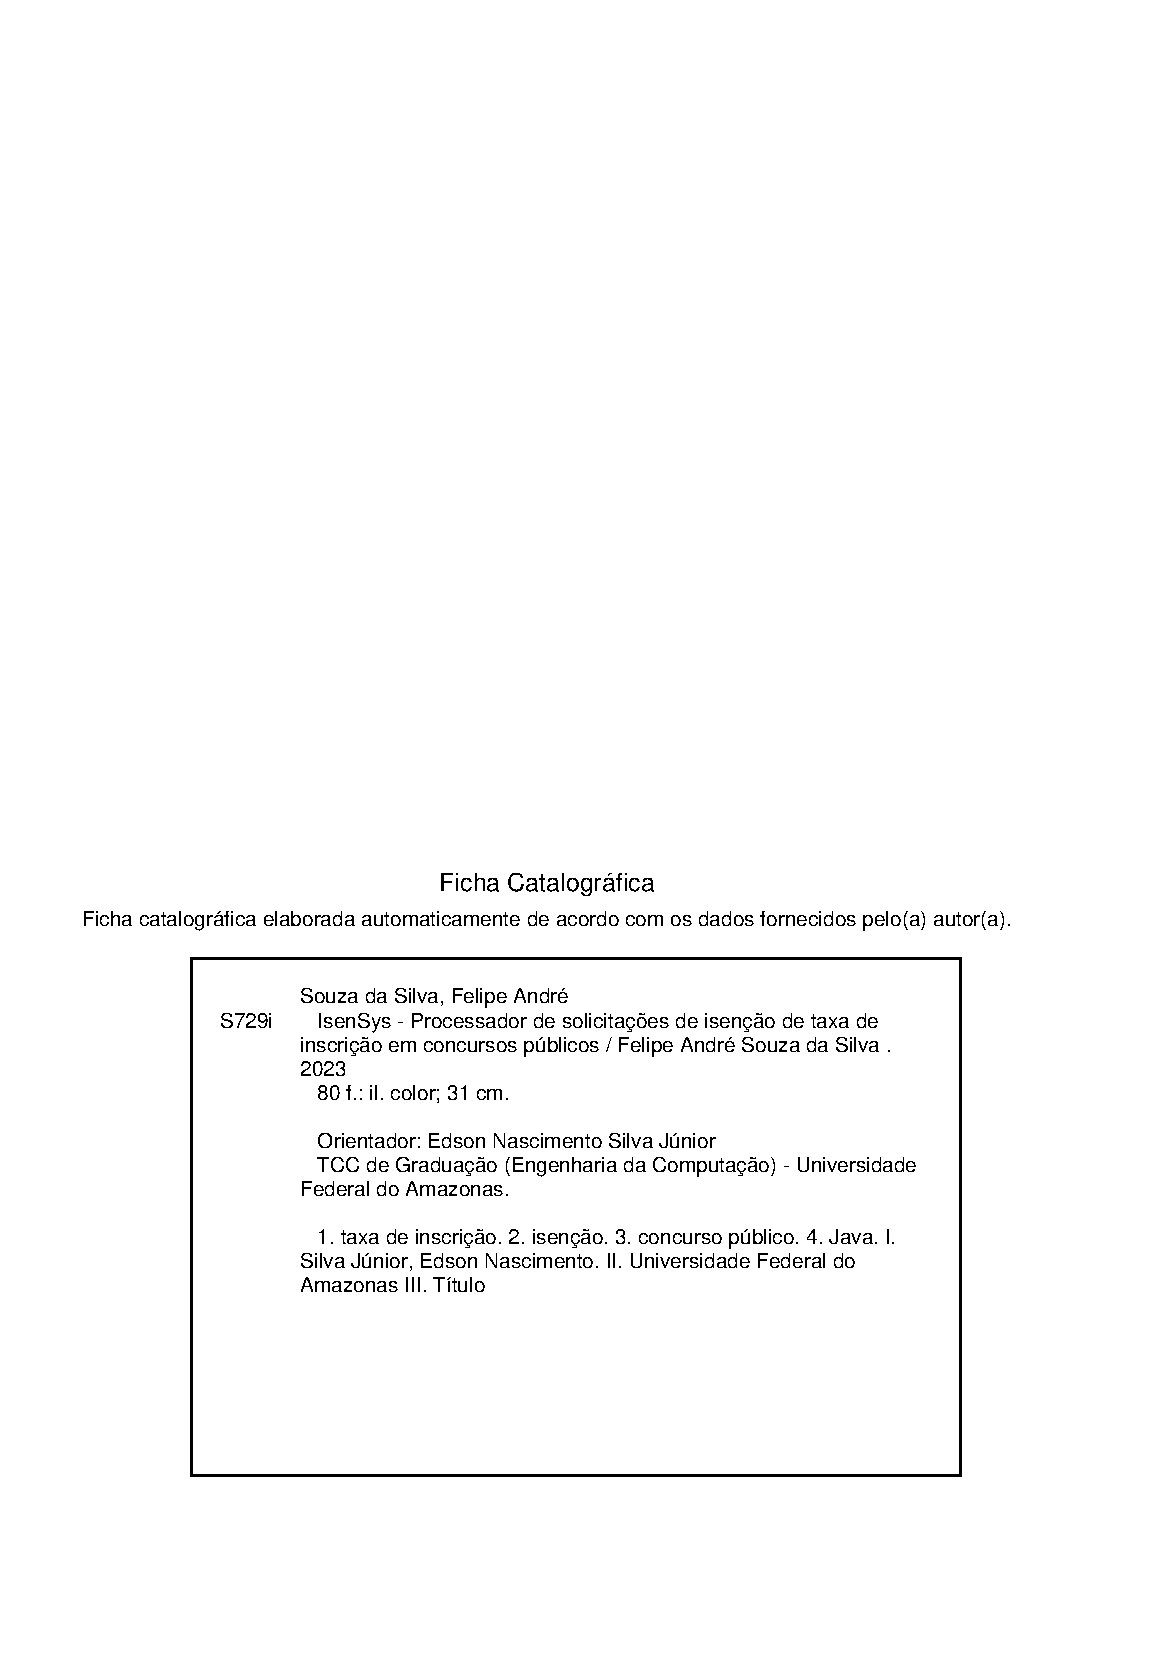
\includepdf{docs/ficha-catalografica}

	% ----------| Folha de Aprovação |----------
	%
	% Isto é um exemplo de Folha de aprovação, elemento obrigatório da NBR
	% 14724/2011 (seção 4.2.1.3). Você pode utilizar este modelo até a aprovação
	% do trabalho. Após isso, substitua todo o conteúdo deste arquivo por uma
	% imagem da página assinada pela banca com o comando abaixo:
	%
	% \includepdf{folhadeaprovacao_final.pdf}
	%
	\begin{folhadeaprovacao}
		\parindent=0pt
		\setlength{\ABNTEXsignskip}{1.5cm}

		Monografia de Graduação sob o título \textit{\imprimirtitulo} apresentada por {\imprimirautor} e aceita pela Faculdade de Tecnologia da {\imprimirinstituicao}, sendo aprovada por todos os membros da banca examinadora abaixo especificada:

		\assinatura{\fontsize{12}{15}\selectfont {\imprimirorientador} \\ \fontsize{11}{15} \selectfont {\fontsize{10}{12}\selectfont Instituto de Computação \par \imprimirinstituicao }}
		\vspace{1cm}
		\assinatura{Dra. Fabíola Guerra Nakamura \\ {\fontsize{10}{12}\selectfont Instituto de Computação \par \imprimirinstituicao}}
		\vspace{1cm}
		\assinatura{Dr. José Francisco Magalhães Netto \\ {\fontsize{10}{12}\selectfont Instituto de Computação \par \imprimirinstituicao}}
		\vfill
		
		\begin{center}
			\fontsize{12}{15}\selectfont
			\vspace*{0.5cm}
			\imprimirlocal, 08 de Novembro de 2023.
			\vspace*{1cm}
		\end{center}
	
	\end{folhadeaprovacao}

	% ----------| Dedicatória |----------
	\begin{dedicatoria}
		
		\vspace*{\fill}
		\noindent
		\leftskip=7cm
		\textit{À minha mãe, mulher guerreira e fonte de inspiração e forças para conclusão deste curso de graduação.}
		\vspace{5cm}
	
	\end{dedicatoria}

	% ----------| Agradecimentos |----------
	\begin{agradecimentos}

		Em primeiro lugar quero agradecer à minha família que é pequena, mas super unida, minha mãe Adriana, aos meus irmãos Anna Beatriz e Maurício Júnior (\textit{in memoriam}) e nossa amiga Nira, pelo amor incondicional, apoio emocional e encorajamento constante que me proporcionaram durante todos esses anos. Vocês são minha âncora e minha maior motivação.
		
		Aos meus grandes amigos: Alexsandro Evangelista, Arianne Kaist, Hítalo Viana, Leonardo Pinheiro, Maurianne Kaist, Milena Lizandra, Munhoz, Naiara, Nilba, Thiago Lima e Will que compartilharam comigo as alegrias, desafios e preocupações deste percurso, agradeço pela amizade, colaboração, apoio mútuo e por não me permitir enlouquecer.
		
		Também expresso minha gratidão ao meu orientador, Prof. Edson Jr. pela orientação, PACIÊNCIA, dedicação e perseverança ao longo deste processo. Suas orientações, \textit{insights} e sua motivação foram fundamentais para o desenvolvimento deste trabalho e para o meu crescimento como acadêmico e profissional.
		
		Por último, mas não menos importante, quero agradecer a todos os membros do corpo docente, distribuídos nos mais diversos departamentos por onde passei como estudante, cujo conhecimento e ensinamentos moldaram minha jornada acadêmica. Suas aulas foram inspiradoras e enriquecedoras, contribuindo muito para meu crescimento acadêmico.
		
		A conclusão deste ciclo não teria sido possível sem a contribuição de cada uma dessas pessoas, e por isso, expresso minha profunda gratidão a todos. O conhecimento adquirido e as experiências vividas durante esta jornada acadêmica são inestimáveis, e estou ansioso para aplicá-los em meu futuro profissional.
		
		Muito obrigado a todos por fazerem parte desta conquista!

	\end{agradecimentos}

	% ----------| Epígrafe |----------
	\begin{epigrafe}
		
		\vspace*{\fill}
		\begin{flushright}
			
			\textit{Software is a great combination between artistry and engineering.}

			\textit{Bill Gates}
			
		\end{flushright}\vspace{4cm}
		
	\end{epigrafe}

	% ----------| Resumo |----------
	\setlength{\absparsep}{18pt}
	\begin{resumo}

		Este documento versa sobre o desenvolvimento de um aplicativo computacional para processar solicitações de isenção de taxa de inscrição em concursos públicos de acordo com as normativas do Ministério do Desenvolvimento Social do Brasil e os interesses da Comissão Permanente de Concursos da UFAM. O sistema, que opera coletivamente com o Sistema de Isenção de Taxa de Concurso, do Ministério do Desenvolvimento Social do Brasil, permite que um órgão gestor prepare dados pessoais de candidatos solicitantes de isenção de taxa de inscrição para envio ao sistema do Ministério do Desenvolvimento e, após o processamento de tais solicitações pelo sistema, gere documentos de publicação de resultados e relatórios com o objetivo de garantir a lisura e transparência deste processo tão democrático. No desenvolvimento foi utilizada a linguagem de programação \textit{Java} e tecnologias de grande consolidação no mercado como o \textit{Jasper Reports}, para geração de relatórios e o \textit{Apache POI}, adicionando suporte a arquivos do \textit{Microsoft Excel}.

		\vspace{\onelineskip}

		\noindent
		\textit{Palavras-chave}: taxa de inscrição, isenção, concurso público, Java.

	\end{resumo}

	% ----------| Abstract |----------
	\begin{abstracteng}[Abstract]
		\begin{otherlanguage*}{english}
		
			This document relates to the development of a computer application that facilitates applying for the waiving of fees when sitting public examinations. This is in accordance with the guidelines set by the Brazilian Ministry of Social Development and the requirements of the UFAM Permanent Commission for Examinations. The app system works with the System of Exemption Fees of the Ministry, allowing anyone concerned to handle the personal data of candidates applying for exemption, in order for it to be sent to the Ministry's system. After this process, it creates a public notice and reports, guaranteeing smoothness and transparency in the democratic process. \textit{Java} programming language was used in the development of the app. Other compatible technologies, such as \textit{Jasper Reports}, was used to generate reports and the \textit{Apache POI}, for the processing of \textit{Microsoft Excel} files.

			\vspace{\onelineskip}
			\noindent
			\textit{Keywords}: examination fee, exemption, public examination, Java.
	
		\end{otherlanguage*}
	\end{abstracteng}

	% ----------| Lista de Figuras |----------
	\pdfbookmark[0]{\listfigurename}{lof}
	\listoffigures*
	\cleardoublepage

	% ----------| Lista de Tabelas |----------
	\pdfbookmark[0]{\listtablename}{lot}
	\listoftables*
	\cleardoublepage

	% ----------| Lista de Abreviaturas e Siglas |----------
	\begin{siglas}

		\item[CadÚnico] Cadastro Único para Programas Sociais do Governo Federal
		\item[CNPJ] Cadastro Nacional de Pessoas Jurídicas
		\item[CSV] \textit{Comma-separated values} - valores separados por vírgula
		\item[COMPEC] Comissão Permanente de Concursos da UFAM
		\item[IDE] \textit{Integrated Development Environment} - ambiente de desenvolvimento integrado
		\item[IRPF] Imposto sobre a Renda das Pessoas Físicas
		\item[IRPJ] Imposto sobre a Renda das Pessoas Jurídicas
		\item[NIS] Número de Identificação Social
		\item[REDOME] Registro Brasileiro de Doadores Voluntários de Medula Óssea
		\item[SISTAC] Sistema de Isenção de Taxa de Concurso
		\item[UFAM] Universidade Federal do Amazonas

	\end{siglas}

	% ----------| Sumário |----------
	\pdfbookmark[0]{\contentsname}{toc}
	\tableofcontents*
	\cleardoublepage

	% ----------| Início dos Elementos Textuais |----------
	\textual

	% ----------| Capítulo 1: Introdução |----------
	\chapter{Introdução}
	
		Com a missão de cultivar o saber em todas as áreas do conhecimento por meio do ensino, pesquisa e da extensão, a Universidade Federal do Amazonas (UFAM) é uma das principais portas de entrada para o desenvolvimento pessoal e intelectual, contando com cerca de 29.000 alunos e 3.400 servidores distribuídos em seis \textit{campi} ao redor do Estado do Amazonas, em 2023.
		
		Tomando como objeto de estudo e inspiração para este trabalho, um setor específico desta universidade foi adotado: a Comissão Permanente de Concursos (COMPEC), que é um órgão suplementar responsável pela execução dos principais processos seletivos de graduação e concursos para provimento de cargos da universidade.
		
		Uma das tarefas mais democráticas e delicadas executadas por este setor é o processo de isenção de pagamento de taxa de inscrição em concursos e processos seletivos.
		
		Atualmente a COMPEC, como qualquer outro órgão do poder executivo do Brasil, adota três tipos de modalidades de isenção: por cadastro no Registro Brasileiro de Doadores Voluntários de Medula Óssea (REDOME), por comprovação de baixa renda e curso de nível médio de forma gratuita e por meio do Cadastro Único para Programas Sociais do Governo Federal (CadÚnico).
		
		Um dos desafios enfrentados pela COMPEC é a gerência e correto processamento das solicitações de isenção, de forma a não prejudicar os candidatos, tampouco a imagem da UFAM e do funcionalismo público. Para ilustrar, apenas em 2023 a COMPEC realizou 10 concursos, mobilizando ao total 39.289 candidatos, dos quais 18.709 solicitaram isenção de taxa de inscrição, onde 8.947 deles tiveram o benefício concedido.
		
		Inicialmente a COMPEC realizava todo o processo de forma artesanal, logo, com o intuito de automatizar e otimizar tal processo, este trabalho apresenta uma aplicação de computador capaz de analisar dados, processar e confeccionar relatórios para publicação, tomando como objeto de estudo a modalidade de isenção mais volumosa em termos de solicitação: a modalidade CadÚnico, regulamentada pelo Decreto n{\textordmasculine} 6.593, de 2 de outubro de 2008 \cite{cadunico-decreto}.
		
		A aplicação, denominada \textit{IsenSys}, procura ainda fornecer uma interface simples e objetiva, com dicas e tratamentos de forma a instruir intuitivamente sua utilização ao usuário, tomando ainda como alicerce no seu desenvolvimento, os cinco princípios fundamentais da Administração Pública do Brasil: legalidade, impessoalidade, moralidade, publicidade e eficiência.

		\section{Objetivos}
		
			\subsection{Objetivo Geral}
			
			Esta monografia possui como objetivo apresentar um aplicativo processador de solicitações de isenção de taxa de inscrição de acordo com a regulamentação do CadÚnico \cite{cadunico-decreto}, de forma a permitir agilidade e acurácia nos resultados, por parte de um órgão gestor do Poder Executivo do Brasil.
			
			\subsection{Objetivos Específicos}
			
			\begin{itemize}
				
				\item Implementar à risca o motor do sistema \textit{(backend)} utilizando as normativas do manual do SISTAC \cite{sistac-formatos}, visando erradicar os erros de processamento dos lotes de envio;
				\item Utilizar das boas práticas de programação para tornar o projeto simples e permitir colaboração;
				\item Implementar uma interface gráfica simples e intuitiva, com dicas e tratamentos de exceções, visando agilidade e fluidez na interação com o sistema.
				
			\end{itemize}
		
		\section{Organização da Monografia}
		
			Esta monografia possui a seguinte estrutura de capítulos:
			
			\begin{itemize}
				
				\item \textbf{Capítulo 2}: aborda os fundamentos teóricos, principais tecnologias e bibliotecas utilizadas no desenvolvimento do \textit{IsenSys};
				\item \textbf{Capítulo 3}: detalha o processo de desenvolvimento do \textit{IsenSys}, por meio de diagramas de alto nível, detalhamento de funcionalidades e exibição da interface gráfica;
				\item \textbf{Capítulo 4}: descreve resultados e métricas que permitem ter um comparativo entre o antes e depois da implementação do \textit{IsenSys};
				\item \textbf{Capítulo 5}: apresenta as considerações finais, conclusão e futuras atualizações no \textit{IsenSys}.
				
			\end{itemize}
	
	% ----------| Capítulo 2: Referencial Teórico |----------
	\chapter{Referencial Teórico}
	
		Este capítulo referencia as principais ferramentas e tecnologias utilizadas no desenvolvimento do \textit{IsenSys}, tais como linguagem de programação, bibliotecas de funções e o ambiente de desenvolvimento. A última seção deste capítulo [\ref{isencao}] explica e detalha o funcionamento do processo de isenção adotado pela COMPEC.
		
		\section{Java}
		
			A linguagem de programação Java \cite{java} é uma das mais bem conceituadas e utilizadas ao redor do mundo. Concebida em meados de 1995 pela empresa \textit{Sun Microsystems}, tem conquistado o mundo pela sua simplicidade, boa curva de aprendizagem, forma de organização e versatilidade entre os vários sistemas operacionais e dispositivos.
		
			Por ser uma linguagem independente de plataforma, ela permite que uma mesma aplicação possa ser executada em diversos equipamentos portando sistemas operacionais de diversas arquiteturas, sem a necessidade de adaptação ou reconstrução de código por parte do desenvolvedor, comportamento que torna suas aplicações escaláveis e robustas.
		
			\begin{figure}[ht]
				\begin{center}
				
					\caption{Logomarca do \textit{Java}}
					
\includegraphics[scale=0.04]{img/java-logo}
					\legend{Fonte: \url{https://www.oracle.com/br/java/technologies/java-se-glance.html}}
					
				\end{center}
			\end{figure}
		
			Atualmente mantida pela empresa \textit{Oracle Corporation}, a linguagem continua sendo livre e gratuita para utilização pessoal e para algumas classes de aplicações, e possui uma rica e extensa comunidade de suporte e documentação. As atualizações regulares também são gratuitas e sempre trazem otimizações, novas funcionalidades e melhorias de segurança.

			Provavelmente o leitor já tenha utilizado algumas das aplicações implementadas utilizando a tecnologia Java, programas como: declaração de imposto sobre a renda (IRPF e IRPJ), Processo Judicial Eletrônico (PJe), \textit{MATLAB}, famoso no mundo da engenharia e até o próprio sistema \textit{Android}, um dos principais sistemas operacionais para dispositivos móveis.
		
		\section{Apache Commons Text\texttrademark} \label{commons-text}
		
			O \textit{Apache Commons Text\texttrademark} \cite{commons-text} é uma biblioteca livre (\textit{open-source}) escrita em linguagem Java, desenvolvida e mantida pela \textit{Apache Software Foundation}, que é uma organização mundial sem fins lucrativos criada para dar suporte de desenvolvimento a projetos de programação de código aberto, ou seja, livres para todos.
			
			A biblioteca oferece funcionalidades para manipulação e processamento de texto, tornando tarefas comuns de manipulação de strings mais eficientes e simples para desenvolvedores Java, algumas são: manipulação e escapamento de \textit{Strings}, algoritmos de distância e similaridade, tokenização, geração de senhas aleatórias, formatação em geral, dentre muitas outras.
		
		\section{Apache Maven} \label{maven}
		
			Até o presente momento foram citadas algumas bibliotecas utilizadas como complemento de código para a linguagem Java, prática muito comum entre os desenvolvedores em qualquer linguagem de programação. Porém, muitas vezes sua gerência pode ser complicada se realizada de forma manual, pois bibliotecas resultam em arquivos, que podem sofrer corrompimento ou passar por atualizações de versão.
		
			O \textit{Apache Maven} \cite{maven} surge como uma ferramenta de gerenciamento e compreensão de projetos escritos em Java, onde é possível organizar bibliotecas e publicá-las de forma gratuita para utilização pela comunidade de desenvolvimento. Podemos esperar também funcionalidades como atualizações, verificação de integridade e autoinstalação.
		
			A utilização deste gerente é muito simples, tendo em vista que muitas suítes de desenvolvimento oferecem suporte nativo ao \textit{Maven}. Após instalada, basta organizar as dependências (bibliotecas) do projeto em um arquivo especifico denominado 'pom.xml', salvar e esperar que o próprio \textit{Maven} configure as bibliotecas no projeto.
			
			\begin{figure}[ht]
				\begin{center}
					
					\caption{Logo do gerente de projetos \textit{Apache Maven}}
					
\includegraphics[scale=0.45]{img/maven-logo}
					\legend{Fonte: \url{https://maven.apache.org}}
					
				\end{center}
			\end{figure}
		
		\section{Apache POI}
		
			O \textit{Apache POI} \cite{poi} também é uma biblioteca gratuita escrita utilizando a linguagem Java, que adiciona suporte de leitura e escrita de dados em documentos do \textit{Microsoft Office} diretamente das aplicações Java, sem a necessidade de aquisição e instalação dos aplicativos da \textit{Microsoft}.
			
			\begin{figure}[ht]
				\begin{center}
					
					\caption{Logo da biblioteca \textit{Apache POI}}
					
\includegraphics[scale=0.3]{img/apache-poi}
					\legend{Fonte: \url{https://poi.apache.org}}
					
				\end{center}
			\end{figure}
		
		\section{Eclipse IDE}
		
			No mundo do desenvolvimento de software, agilidade e escalabilidade estão entre as qualidades mais requisitadas nas linguagens. Como forma de satisfazer tais demandas, existe no mercado uma vasta gama do que chamamos de \textit{IDE - integrated development environment} ou ambiente de desenvolvimento integrado, amplamente aceitos pela comunidade.
			
			Inicialmente o projeto \textit{Eclipse} \cite{eclipse} foi concebido pensando no desenvolvimento utilizando a linguagem Java, mas atualmente suporta extensões \textit{(plugins)} que adicionam suporte a várias outras linguagens, tais como \textit{PHP}, \textit{Python}, \textit{Arduino} etc e ainda, por ser de código aberto, pode ser modificado para outras finalidades.
			
			O aplicativo adiciona funcionalidades que auxiliam muito no desenvolvimento em uma linguagem, tais como autocomplemento de código, exibição de sugestões, dicas e tratamentos de erros, verificador de sintaxe e semântica e até integração com outras tecnologias como versionadores de código e o \textit{Apache Maven} [\ref{maven}].
			
			\begin{figure}[ht]
				\begin{center}
					
					\caption{\textit{Eclipse IDE}}
					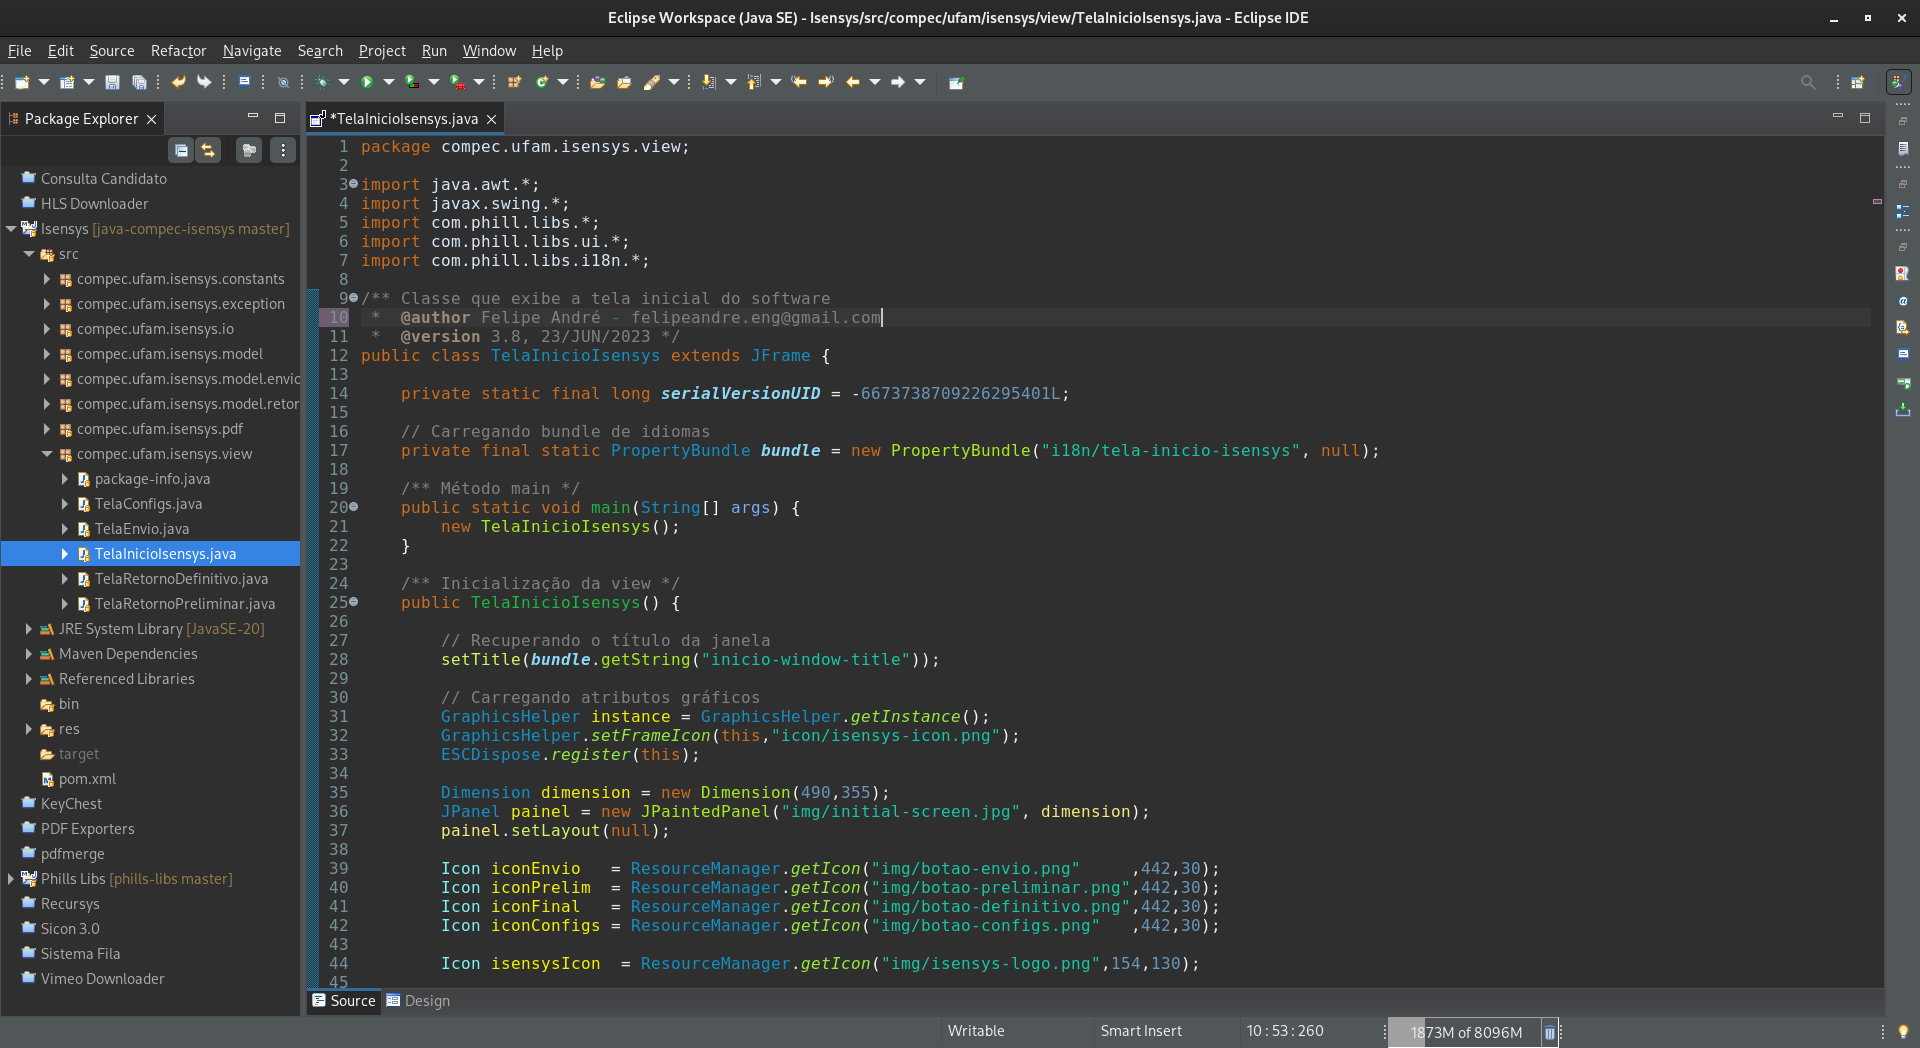
\includegraphics[scale=0.2]{img/eclipse-ide}
					
				\end{center}
			\end{figure}
		
		\section{JasperReports\textregistered}
		
			A biblioteca \textit{JasperReports\textregistered} \cite{jasper} é gratuita e uma das mais robustas e populares utilizadas para criação de relatórios para aplicações escritas em Java. Possui sua própria suíte de design, onde o desenvolvedor pode rapidamente configurar um novo relatório com poucos passos, seguindo guias e instruções diretamente na interface gráfica do editor.
			
			Por ser desenvolvida utilizando a linguagem Java, ela também apresenta o mesmo comportamento e visualização em qualquer sistema operacional onde está disponível, produzindo relatórios de alta qualidade e escalabilidade, oferecendo opções de exportação para outros formatos conhecidos, tais como \textit{PDF}, \textit{Web} e \textit{Microsoft Word}.
			
			\begin{figure}[ht]
				\begin{center}
				
				\caption{Suíte de desenvolvimento \textit{JasperReports\textregistered}}
				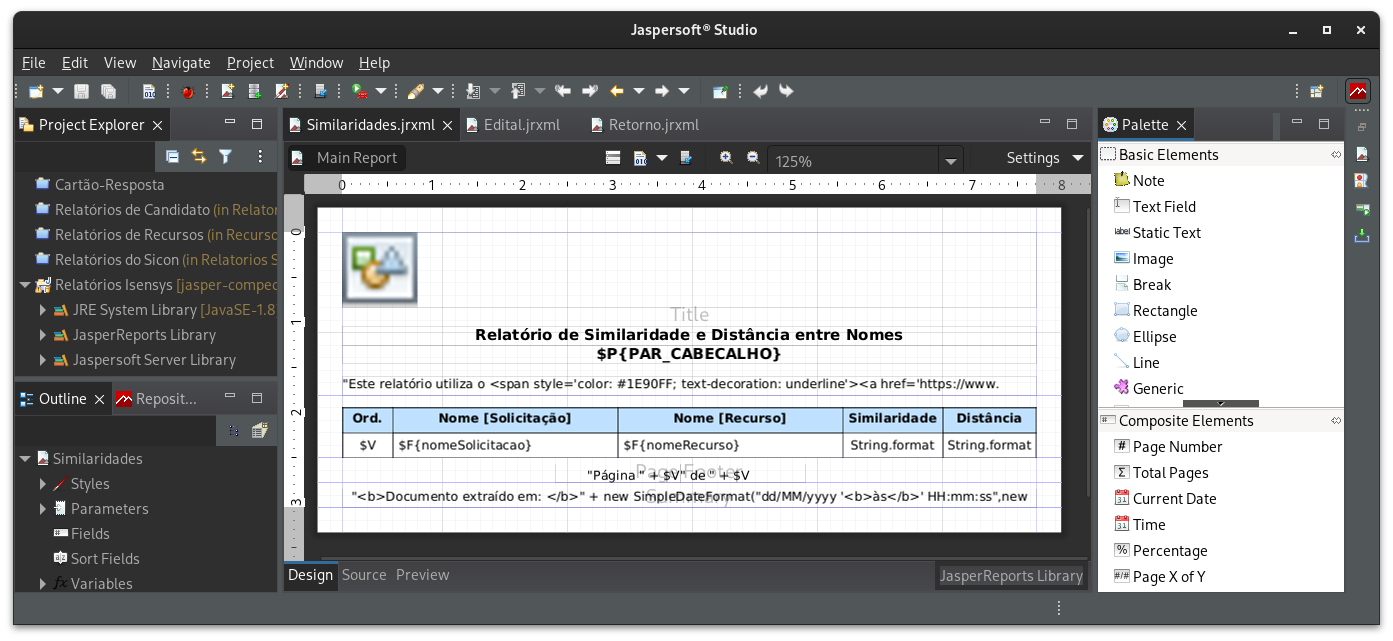
\includegraphics[scale=0.35]{img/jaspersoft}
				
				\end{center}
			\end{figure}
			
		\section{\textit{Jaro-Winkler}} \label{jaro-winkler}
		
			O algoritmo de \textit{Jaro-Winkler} \cite{jaro-winkler} é uma técnica de comparação de strings que mede a semelhança entre duas sequências de caracteres. Ele é frequentemente utilizado para encontrar correspondências aproximadas entre strings, especialmente em aplicações de deduplicação de dados e pesquisa de registros. A seguir, encontra-se um resumo da implementação do algoritmo.
			
			Dados: Duas strings, $s_1$ e $s_2$
			
			\noindent
			\textbf{Passo 1:} Encontre o comprimento das strings:
			\[
			\text{len}_1 = \text{comprimento}(s_1)
			\]
			\[
			\text{len}_2 = \text{comprimento}(s_2)
			\]
			
			\noindent
			\textbf{Passo 2:} Defina o valor de $m$ como o número de caracteres em comum (correspondentes) entre as duas strings, considerando uma janela de proximidade:
			\[
			\text{Janela} = \left\lfloor\max(\text{len}_1, \text{len}_2) / 2\right\rfloor - 1
			\]
			
			\[
			\text{m} = \text{número de caracteres em comum dentro da janela}
			\]
			
			\noindent
			\textbf{Passo 3:} Calcule o número de transposições:
			\[
			\text{t} = \frac{1}{2} \times \left(\text{número de transposições de caracteres entre $s_1$ e $s_2$}\right)
			\]
			
			\noindent
			\textbf{Passo 4:} Calcule a medida de similaridade de Jaro:
			\[
			\text{Jaro\_Sim} = \frac{m}{\text{len}_1} + \frac{m}{\text{len}_2} + \frac{m - t}{m}
			\]
			
			\noindent
			\textbf{Passo 5:} Calcule o fator de ajuste de prefixo Winkler:
			\[
			\text{Prefix\_Factor} = 0
			\]
			\[
			\text{Prefix\_Len} = \text{número de caracteres idênticos no início das strings}
			\]
			
			Se $\text{Prefix\_Len} > 4$, limite $\text{Prefix\_Len}$ a 4.
			
			\[
			\text{Prefix\_Factor} = \text{Prefix\_Len} \times 0.1 \times (1 - \text{Jaro\_Sim})
			\]
			
			\noindent
			\textbf{Passo 6:} Calcule a medida de similaridade de Jaro-Winkler:
			\[
			\text{Jaro\_Winkler\_Sim} = \text{Jaro\_Sim} + \text{Prefix\_Factor}
			\]
			
			\noindent
			\textbf{Passo 7:} A medida de similaridade final entre $s_1$ e $s_2$ é dada por $\text{Jaro\_Winkler\_Sim}$.
			
			O valor resultante de $\text{Jaro\_Winkler\_Sim}$ está dentro do intervalo [0, 1], onde 0 indica nenhuma semelhança e 1 indica correspondência perfeita. Quanto maior o valor, maior a semelhança entre as duas strings.
			
		\section{Joda-Time}
			
			A biblioteca \textit{Joda-Time} \cite{joda-time} facilita praticamente qualquer operação e manipulação com datas em um sistema Java, tarefa que é deveras complicada utilizando apenas os recursos nativos da linguagem. Com uma boa documentação e as mais diversas classes para cálculos, formatação e operações com data, tem conquistado muitos desenvolvedores a utilizá-la em seus projetos.
			
			Felizmente, \textit{Joda-Time} é uma biblioteca livre para utilização pessoal e comercial, licenciada sobre a \textit{Licença Apache 2.0}. Também é considerada consolidada e estável, estando até os dias atuais recebendo atualizações de otimização e novas funcionalidades.

		\section{Processo de Isenção} \label{isencao}
		
			Compreender o processo de isenção de taxa de inscrição é parte fundamental para entender a importância e seriedade empenhados no desenvolvimento do \textit{IsenSys}. Durante esta seção, serão abordadas de forma detalhada e objetiva as fases e o \textit{modus operandi} do processamento das solicitações de isenção de taxa de inscrição, a ser referenciada no decorrer da monografia apenas como \textit{solicitações de isenção} ou ainda \textit{solicitações}.
		
			A implementação do processo de isenção de taxa de inscrição a candidatos de concursos e processos seletivos por parte da COMPEC, segue as normativas impostas do Decreto n{\textordmasculine} 6.593, de 2 de outubro de 2008 \cite{cadunico-decreto} e no manual de envio e recebimento de solicitações de inscrição do SISTAC \cite{sistac-formatos}.
			
			Como fonte de insumo e também como entrega do resultado final, o sistema denominado "PSConcursos", da UFAM foi utilizado. É ele quem concentra dados dos candidatos a concursos da universidade bem como solicitações de isenção e inscrição. O \textit{IsenSys}, por sua vez, é capaz de importar as solicitações geradas pelo PSConcursos e realizar seu trabalho.
			
			Em cada edital regido pela COMPEC, o processo de isenção é a primeira etapa a ser realizada e sua operacionalização respeita o seguinte fluxo:
			
			\begin{enumerate}
				
				\item \textbf{Publicação de Edital:} onde são definidas as regras gerais do concurso ou processo seletivo;
				\item \textbf{Período de Solicitação de Isenção [1{\textordfeminine} instância]:} geralmente dois dias úteis, onde os candidatos que têm interesse em solicitar isenção, o fazem por meio do preenchimento de um formulário de solicitação no sistema PSConcursos;
				\item \textbf{Período de Análise:} é o tempo que a COMPEC possui para processar as solicitações, geralmente entre 3 a 4 dias úteis. O PSConcursos disponibiliza um arquivo \textit{csv} com todas as solicitações obtidas no período editalício, insumo para envio ao SISTAC que, por sua vez, analisa as solicitações e retorna também um arquivo \textit{csv}, útil para a confecção do resultado preliminar;
				\item \textbf{Publicação do Resultado Preliminar:} aqui é tornado público o resultado do processamento das solicitações em 1{\textordfeminine} instância;
				\item \textbf{Período de Recurso [2{\textordfeminine} instância]:} é a oportunidade que o candidato que teve sua solicitação indeferida em 1{\textordfeminine} instância, recursar, preenchendo um formulário de recurso no sistema PSConcursos. Vale ressaltar que só podem recursar os candidatos que solicitaram isenção em 1{\textordfeminine} instância!
				\item \textbf{Período de Análise:} é o tempo que a COMPEC possui para processar os recursos, geralmente entre 2 a 3 dias úteis. Aqui é realizado o mesmo processo descrito no primeiro período de análise;
				\item \textbf{Publicação do Resultado Definitivo:} publicação do resultado definitivo, juntamente com a carga de informações no PSConcursos, encerrando o processo de isenção.
				
			\end{enumerate}
			
			O fluxograma a seguir ilustra de uma forma mais concisa este processo.
			
			\begin{figure}[ht]
				\begin{center}
					
					\caption{Fluxograma das Etapas de Isenção}
					
					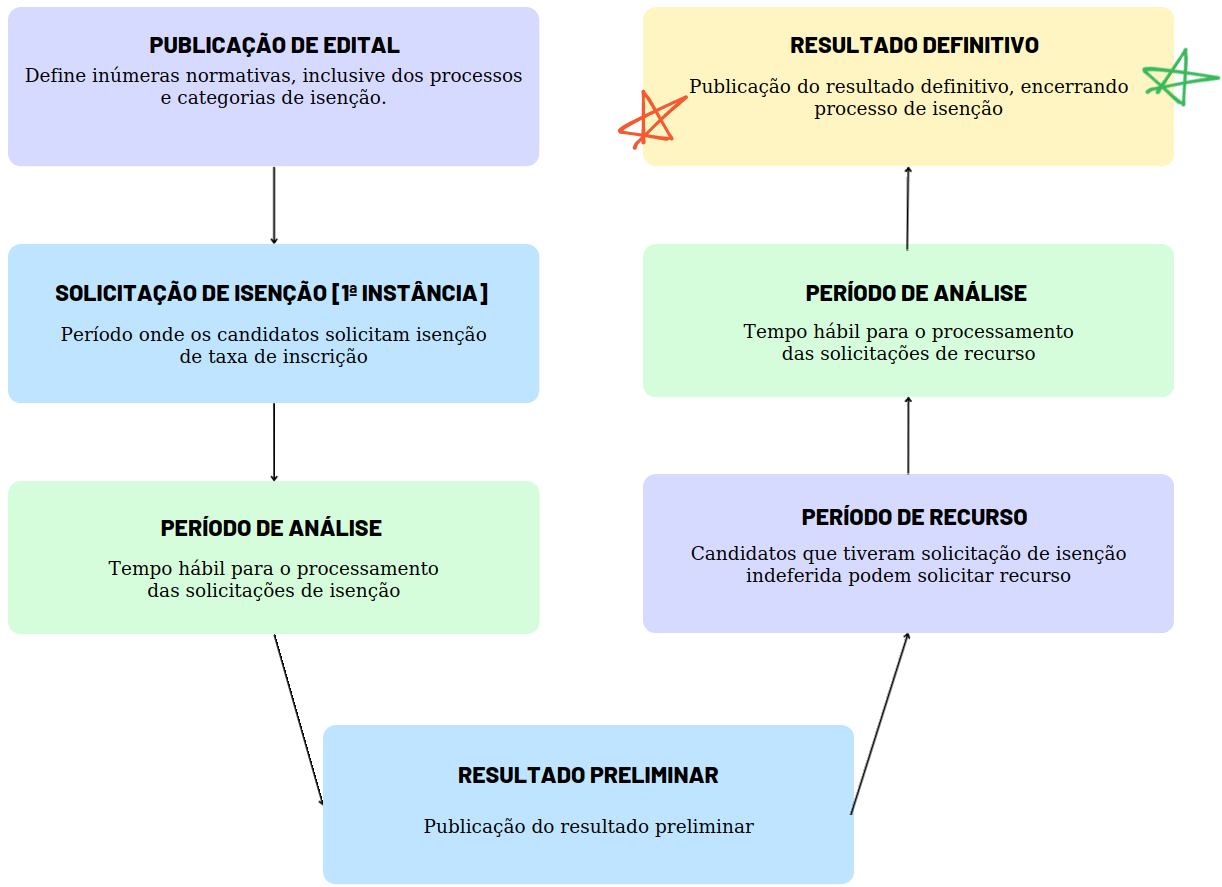
\includegraphics[scale=0.37]{img/isencao-fluxograma}
					
				\end{center}
			\end{figure}

	% ----------| Capítulo 3: Desenvolvimento do IsenSys |----------
	\chapter{Desenvolvimento do \textit{IsenSys}}

		Introduzidas as principais ferramentas utilizadas no projeto, aprofundar-se-á no processo de desenvolvimento do aplicativo \textit{IsenSys}. Conceitos como especificações de sistema, requisitos para utilização e formas de aplicação serão demonstrados de maneira objetiva.
		
		O desenvolvimento do motor do sistema (\textit{backend}) é regido pelas normas de formato de arquivo e diretivas definidas no documento de orientações gerais do SISTAC \cite{sistac-gerais} e no manual de envio e recebimento de arquivos \cite{sistac-formatos}, versão 10.0, publicada em 24/06/2016.
		
		Os requisitos funcionais (RF) do sistema são:
	
		\begin{itemize}

			\item O sistema deverá permitir a importação de dados de candidatos através de arquivos do tipo \textit{csv} ou planilhas do \textit{Microsoft Excel} (RF01);
			\item O sistema deverá permitir o cadastro e edição de dados do órgão gestor (RF02);
			\item O sistema deverá realizar testes de integridade nos dados de solicitações importadas (RF03);
			\item O sistema deverá gerar arquivos de importação para o SISTAC (RF04);
			\item O sistema só pode entregar um arquivo de importação com os dados de solicitações em sua plena completude e integridade (RF05);
			\item Dados de solicitações que foram informadas de forma incompleta ou inválida serão considerados erros e deverão ser exportados em uma planilha (RF06);
			\item O sistema deverá permitir a importação do arquivo de retorno do SISTAC (RF07);
			\item A partir do arquivo de retorno do SISTAC, o sistema deverá produzir relatórios prontos para análise e publicação (RF08);
			\item O sistema também deve permitir a importação da planilha com erros, para inclusão nos relatórios públicos (RF09);
			\item O sistema deve gerar relatórios de estatísticas de solicitações deferidas e indeferidas (RF10);
			\item O sistema deverá gerar um relatório de similaridade entre nomes de candidatos recursantes (RF11).
			
		\end{itemize}
	
		Os requisitos não-funcionais (RF) do sistema são:
	
		\begin{itemize}
			
			\item A linguagem \textit{Java Standard Edition (Java SE)} foi utilizada no desenvolvimento da aplicação (RNF01);
			\item A versão mínima da \textit{Java Virtual Machine (JVM)} a ser utilizada é a 15 (RNF02);
			\item A suíte de interface gráfica utilizada é o \textit{Java Swing} (RNF03);
			\item Por questões de simplicidade, todas as telas foram construídas utilizando layout absoluto com janela não redimensionável (RNF04);
			\item A versão do \textit{Apache POI} utilizada é a 5.2.3, lançada em 17/09/2022 (RNF05);
			\item A versão do \textit{JasperReports\textregistered} utilizada é a 6.26.0, lançada em 11/09/2023 (RNF06);
			\item O sistema pode ser executado em qualquer computador com suporte mínimo ao \textit{Java Runtime Environment - JRE 15}, mínimo de 1GB de memória RAM disponível e monitor com resolução mínima de 800x600 (RNF07);
			\item Como limitação do \textit{JRE 15}, somente máquinas com arquitetura de CPU de 64-bits são suportadas pelo sistema (RNF08).
			
		\end{itemize}
	
		O sistema conta com três módulos distintos: um dedicado a preparar os dados de candidatos para envio ao SISTAC e os outros dois dedicados a processar os arquivos de retorno do SISTAC e produzir relatórios de publicação preliminar e definitivo. A seguir estão ilustrados os diagramas de atividades do sistema, trazendo uma visão geral do funcionamento do \textit{IsenSys}.
		
		\clearpage
		\begin{figure}[ht]
			\begin{center}
				
				\caption{Diagrama de Atividades do Módulo de Envio}
				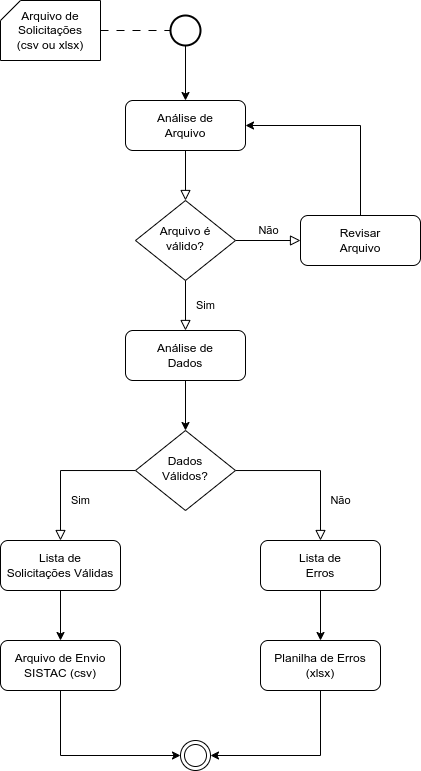
\includegraphics[scale=0.75]{img/diagrama-ativs-envio}
				
			\end{center}
		\end{figure}
		
		\clearpage
		\begin{figure}[ht]
			\begin{center}
				
				\caption{Diagrama de Atividades do SISTAC}
				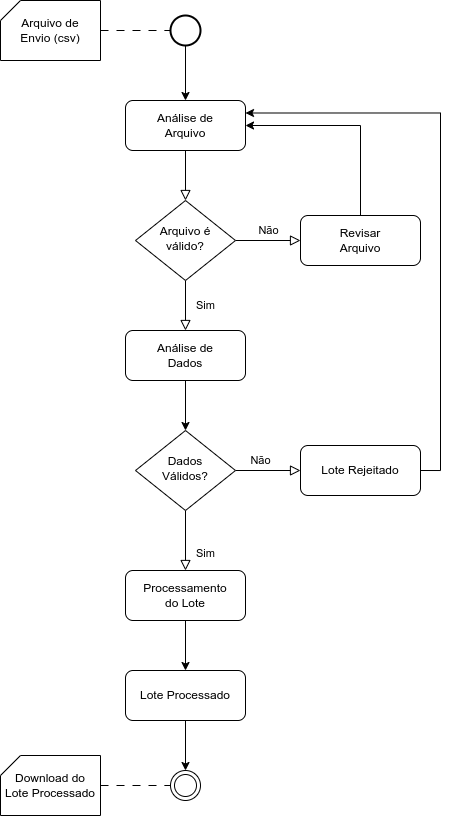
\includegraphics[scale=0.75]{img/diagrama-ativs-sistac}
				
			\end{center}
		\end{figure}
		
		\clearpage
		\begin{figure}[ht]
			\begin{center}
				
				\caption{Diagrama de Atividades do Módulo de Retorno Preliminar}
				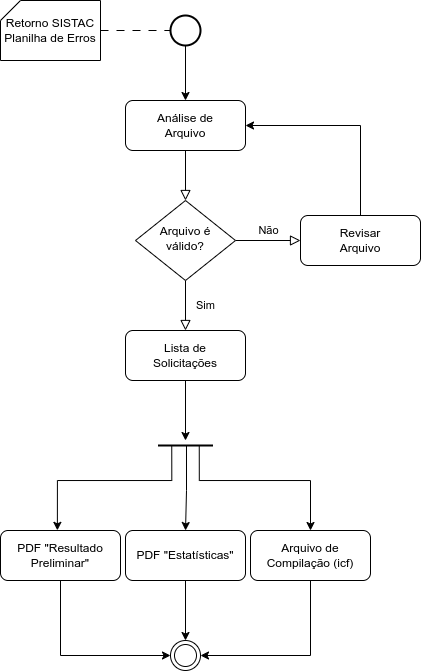
\includegraphics[scale=0.85]{img/diagrama-ativs-prelim}
				
			\end{center}
		\end{figure}
		
		\clearpage
		\begin{figure}[ht]
			\begin{center}
				
				\caption{Diagrama de Atividades do Módulo de Retorno Definitivo}
				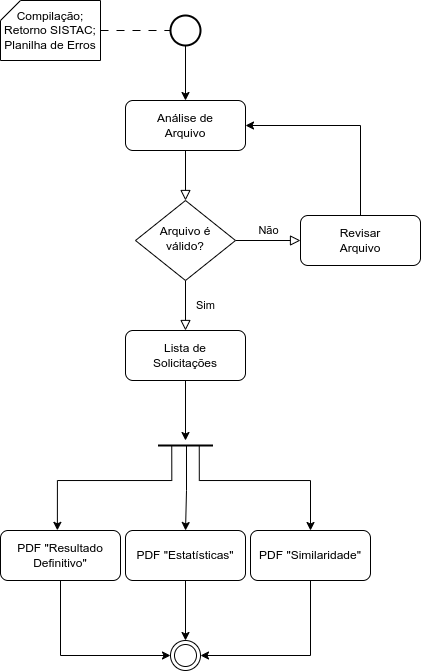
\includegraphics[scale=0.85]{img/diagrama-ativs-definitivo}
				
			\end{center}
		\end{figure}
		
		\clearpage
		\begin{figure}[ht]
			\begin{center}
				
				\caption{Diagrama de Casos de Uso do \textit{IsenSys}}
				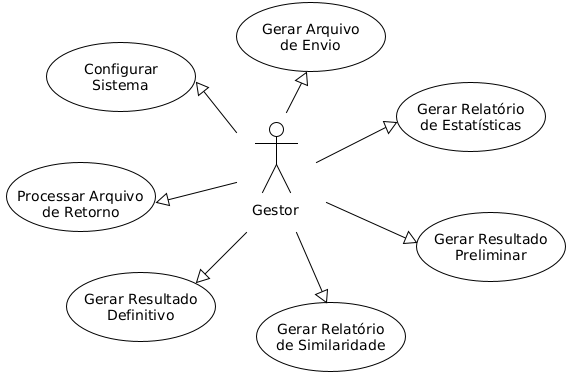
\includegraphics[scale=0.5]{img/casos-uso-isensys}
				
			\end{center}
		\end{figure}
		
		As seções a seguir contém um estudo mais aprofundado sobre a implementação de cada módulo.

		\section{Tela Inicial}
		
			A tela inicial do \textit{IsenSys} agrupa botões que dão acesso a todas as funcionalidades implementadas no sistema. Na primeira utilização é recomendável que o usuário configure os dados do órgão gestor, por meio do botão 'Configurações do Sistema'. A figura a seguir mostra a tela inicial do \textit{IsenSys}.
			
			\begin{figure}[ht]
				\begin{center}
					
					\caption{Tela Inicial do \textit{IsenSys}}
					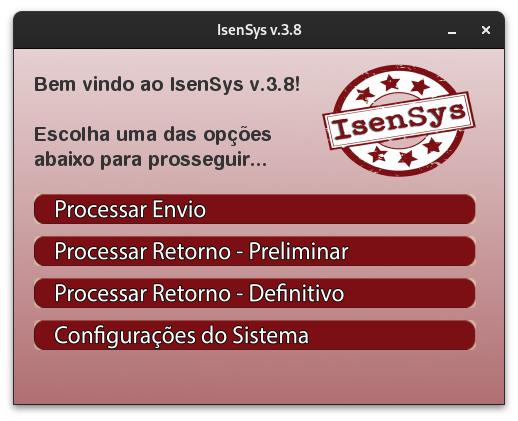
\includegraphics[scale=0.5]{img/inicial}
					
				\end{center}
			\end{figure}

		\section{Tela de Configurações do Sistema}
		
			Algumas configurações são necessárias para o correto funcionamento do \textit{IsenSys}. São elas:
			
			\begin{itemize}
				
				\item \textbf{CNPJ:} indica o número de CNPJ do órgão gestor;
				\item \textbf{Nome Fantasia:} indica o nome fantasia do órgão gestor, contendo no máximo 100 caracteres, segundo o manual do SISTAC \cite{sistac-formatos};
				\item \textbf{Razão Social:} indica a razão social do órgão gestor, também contendo no máximo 100 caracteres, segundo o manual do SISTAC \cite{sistac-formatos};
				\item \textbf{Índices da Planilha de Importação:} indica os índices dos campos de dados dispostos no arquivo de importação de solicitações. Tais índices começam em '0' e vão incrementando a cada coluna. Tomando como exemplo um arquivo de importação do \textit{Microsoft Excel}, a coluna 'A', tem o índice '0', a coluna 'C' tem o índice '2' e assim sucessivamente. Todos os índices devem ser preenchidos.
				
			\end{itemize}
			
			As configurações são salvas em um arquivo binário contido no diretório de recursos do sistema [\ref{recursos}], sob o caminho '\textit{config/program.dat}'.

			\begin{figure}[ht]
				\begin{center}
					
					\caption{Tela de Configurações do Sistema}
					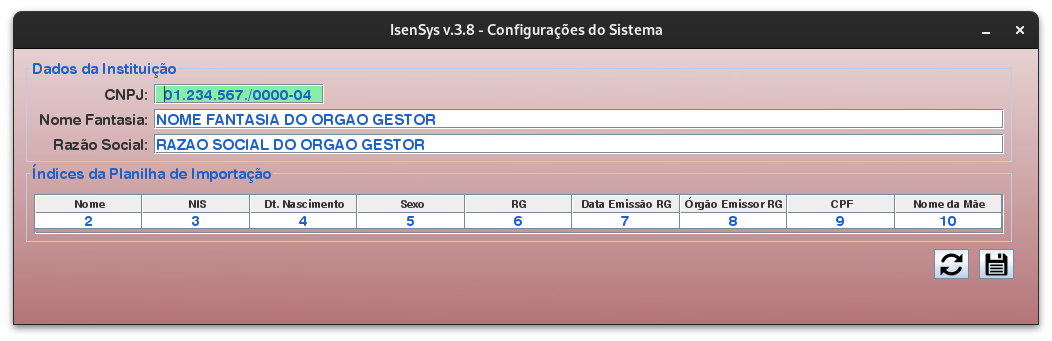
\includegraphics[scale=0.45]{img/configs-ui}
					
				\end{center}
			\end{figure}

		\clearpage
		\section{Desenvolvimento do Módulo de Envio}
	
			Esta seção tem por objetivo detalhar o desenvolvimento do motor \textit{(backend)} de preparação de dados de solicitações de isenção para envio ao SISTAC. Primeiramente precisamos entender como está distribuído o fluxo de informações pelo sistema. Para isto, serão detalhadas as entidades principais e auxiliares deste módulo.
	
			\subsection{Modelagem de um Candidato} \label{candidato}
	
				Os dados pessoais de um candidato são o objeto principal deste sistema, pois compõem uma solicitação de isenção que, após análise pelo SISTAC, tem uma resposta de deferimento ou não. Segundo o manual do SISTAC \cite{sistac-formatos}, os dados pessoais de candidatos necessários para o processamento estão dispostos na tabela a seguir.

				% Tabela gerada com o auxílio da aplicação: https://www.tablesgenerator.com/latex_tables
				\begin{table}[ht]
				
					\caption{Dados pessoais de candidatos e seus formatos}
				
					\begin{tabular}{|c|l|c|c|c|}
						\hline
						\textbf{Campo} & \multicolumn{1}{c|}{\textbf{Descrição}} & \textbf{\begin{tabular}[c]{@{}c@{}}Máximo de\\ Caracteres\end{tabular}} & \textbf{Tipo} & \textbf{Formato} \\ \hline
						Nome & \begin{tabular}[c]{@{}l@{}}Nome completo do candidato\\ sem caracteres especiais e\\ sem abreviações\end{tabular} & 100 & Texto &  \\ \hline
						NIS & \begin{tabular}[c]{@{}l@{}}Número de identificação social\\ do candidato\end{tabular} & 11 & Numérico &  \\ \hline
						\begin{tabular}[c]{@{}c@{}}Data de\\ Nascim.\end{tabular} & \begin{tabular}[c]{@{}l@{}}Data de nascimento do\\ candidato\end{tabular} & 8 & Numérico & ddmmaaaa \\ \hline
						Sexo & Sexo do candidato & 1 & Texto & M ou F \\ \hline
						RG & \begin{tabular}[c]{@{}l@{}}Número do Documento de\\ Identidade do candidato\end{tabular} & 16 & \begin{tabular}[c]{@{}c@{}}Alfanu-\\ mérico\end{tabular} &  \\ \hline
						\begin{tabular}[c]{@{}c@{}}Data de\\ Emissão\end{tabular} & \begin{tabular}[c]{@{}l@{}}Data de emissão do Documen-\\ to de Identidade\end{tabular} & 8 & Numérico & ddmmaaaa \\ \hline
						Sigla RG & \begin{tabular}[c]{@{}l@{}}Sigla do órgão emissor do\\ Documento de Identidade\end{tabular} & 30 & \begin{tabular}[c]{@{}c@{}}Alfanu-\\ mérico\end{tabular} &  \\ \hline
						CPF & Número do CPF do candidato & 11 & Numérico &  \\ \hline
						\begin{tabular}[c]{@{}c@{}}Nome\\ da Mãe\end{tabular} & \begin{tabular}[c]{@{}l@{}}Nome completo da mãe do\\ candidato, sem caracteres\\ especiais e sem abreviações\end{tabular} & 100 & Texto &  \\ \hline
					\end{tabular}
					
				\end{table}
	
				De posse dos dados e tipos, foi concebida a modelagem da entidade \textit{Candidato}, de acordo com o diagrama a seguir.

				% Tabela gerada com o auxílio da aplicação: https://www.tablesgenerator.com/latex_tables
				\begin{figure}[ht]
					\begin{center}
						
						\caption{Modelagem da entidade \textit{Candidato}}
						
						\begin{tabular}{|l|}
							\hline
							\multicolumn{1}{|c|}{\textbf{Candidato}} \\ \hline
							+nome: String \\
							+nis: String \\
							+dataNascimento: DateTime \\
							+sexo: char \\
							+rg: String \\
							+dataEmissaoRG: DateTime \\
							+orgaoEmissorRG: String \\
							+cpf: String \\
							+nomeMae: String \\ \hline
							\\ \hline
						\end{tabular}
						
					\end{center}
				\end{figure}
				
				De acordo com o diagrama de classe da entidade \textit{Candidato}, nota-se que esta apenas armazena dados. As validações nos campos são garantidas por uma classe intermediária, detalhada na seção seguinte.
	
			\subsection{A classe \textit{CandidatoBuilder}} \label{candidato-builder}
				
				Esta classe é responsável por montar um \textit{Candidato} com os dados extraídos de um arquivo de entrada. Durante esse processo ela realiza uma série de validações nos dados, e caso haja pelo menos uma inconsistência, uma exceção com detalhes desta inconsistência é lançada, caso contrário, significa que foi possível construir um objeto respeitando todos os requisitos de formatos do SISTAC \cite{sistac-formatos}. Segue o diagrama de classe do \textit{CandidatoBuilder}.
				
				% Tabela gerada com o auxílio da aplicação: https://www.tablesgenerator.com/latex_tables
				\begin{figure}[ht]
					\begin{center}
						
						\caption{Diagrama de Classe de \textit{CandidatoBuilder}}
						
						\begin{tabular}{|l|}
							\hline
							\multicolumn{1}{|c|}{\textbf{CandidatoBuilder}} \\ \hline
							\\ \hline
							+build() \\
							+parseNome() \\
							+parseNIS() \\
							+parseData() \\
							+parseSexo() \\
							+parseRG() \\
							+parseOrgao() \\
							+parseCPF() \\ \hline
						\end{tabular}
					
					\end{center}
				\end{figure}
	
				Os métodos \textit{parse...()}, são responsáveis por realizar validações específicas em cada campo de dados de um \textit{Colaborador} e lançam exceções detalhadas para que, posteriormente, tanto o órgão gestor dos dados quanto o candidato possam ter conhecimento de quais campos enviaram fora de formato e se ainda cabe algum recurso. Eis a metodologia implementada em cada campo de uma solicitação:
				
				\begin{itemize}
					
					\item \textbf{Nome [candidato e mãe]:} são removidos acentos, cedilhas, múltiplos espaços e quaisquer outros caracteres que não sejam alfabéticos. Se após o processamento, o nome for vazio ou possuir mais que 100 caracteres, um erro é gerado neste campo;
					\item \textbf{NIS:} o número de identificação social (NIS) pode ser verificado pr meio de um algoritmo que utiliza os próprios dígitos de verificação do NIS para validá-lo. No \textit{IsenSys}, esta implementação consta na biblioteca \textit{Phills Libs} \cite{phills-libs}. Caso o algoritmo não consiga validar o NIS, um erro é gerado nesse campo;
					\item \textbf{Data [nascimento e emissão de RG]:} se uma data vazia ou inválida for informada, a data de "01/01/2000"\space é inferida, logo, erros não são gerados nesse campo;
					\item \textbf{Sexo:} caso o sexo informado não seja 'M' ou 'F', um erro é gerado nesse campo;
					\item \textbf{N{\textordmasculine} de RG:} são extraídos apenas caracteres alfanuméricos e, caso a resultante seja vazia ou possuir mais que 16 caracteres, um erro é gerado nesse campo;
					\item \textbf{Órgão Emissor:} são extraídos apenas caracteres alfanuméricos e, caso a resultante seja vazia ou possuir mais que 30 caracteres, o órgão "SSP"\space é inferido, logo, erros não são gerados nesse campo;
					\item \textbf{CPF:} o número de CPF pode ser verificado por meio de um algoritmo que utiliza os próprios dígitos de verificação do CPF para validá-lo. No \textit{IsenSys}, esta implementação consta na biblioteca \textit{Phills Libs} \cite{phills-libs}. Caso o algoritmo não consiga validar o CPF, um erro é gerado nesse campo.
					
				\end{itemize}
				
				Para registrar inconsistências em cada um dos campos de dados de um \textit{Candidato}, é utilizada a classe de exceção \textit{FieldParseException} que, por sua vez, é incorporada à classe de exceção \textit{RowParseException}, montada com todas as exceções percebidas pelo método \textit{build()}.

			\subsection{A classe de exceção \textit{FieldParseException}}
	
				Como forma de descentralizar as tratativas de validação de dados de candidatos, a classe de exceção \textit{FieldParseException} é responsável por armazenar informações sobre o motivo de um campo não ter sido validado e qual campo gerou esta exceção. Esta classe estende a superclasse \textit{Exception} e monta uma \textit{String} formatada com o motivo e o nome do campo inválido.

			\subsection{A classe de exceção \textit{RowParseException}}	

				Com o objetivo de concentrar todas as exceções de validação dos campos de dados de um \textit{Candidato}, a classe de exceção \textit{RowParseException} armazena tais exceções em uma lista encadeada e ainda adiciona informações que ajudam a identificar qual foi a solicitação que gerou a(s) exceção(ões) e ainda em qual posição do arquivo de entrada ele está.
	
				A seguir é possível visualizar o diagrama de classe de \textit{RowParseException}.
	
				% Tabela gerada com o auxílio da aplicação: https://www.tablesgenerator.com/latex_tables
				\begin{figure}[ht]
					\begin{center}
						
						\caption{Diagrama de Classe de \textit{RowParseException}}
			
						\begin{tabular}{|l|}
							\hline
							\multicolumn{1}{|c|}{\textbf{RowParseException}} \\ \hline
							+linha: int \\
							+nis: String \\
							+cpf: String \\
							+nome: String \\
							+listaExcecoes: List\textless{}FieldParseException\textgreater{} \\ \hline
							+addException() \\
							+hasException() \\
							+getMessage() \\
							+getErrorSummaryArray() \\
							+getErrorSummaryString() \\ \hline
						\end{tabular}
						
					\end{center}
				\end{figure}

			\subsection{A classe \textit{ParseResult}} \label{parse-result}
	
				Esta classe é responsável por concentrar o resultado da extração de dados do(s) arquivo(s) de entrada em duas listas:
		
				\begin{enumerate}
						
					\item \textbf{Lista de \textit{Candidato}:} onde são armazenados apenas dados de candidatos solicitantes de isenção que passaram com sucesso por todas as validações de campos definidas na classe \textit{CandidatoBuilder} [\ref{candidato-builder}];
					\item \textbf{Lista de \textit{RowParseException}:} onde são armazenados os dados de solicitações julgados inválidos pela classe \textit{CandidatoBuilder} [\ref{candidato-builder}].
						
				\end{enumerate}
	
				A seguir podemos compreender melhor a classe por meio de seu diagrama.
	
				% Tabela gerada com o auxílio da aplicação: https://www.tablesgenerator.com/latex_tables
				\begin{figure}[ht]
					\begin{center}
						
						\caption{Diagrama de Classe de \textit{ParseResult}}
						
						\begin{tabular}{|l|}
							\hline
							\multicolumn{1}{|c|}{\textbf{ParseResult}} \\ \hline
							+listaCandidatos: List\textless{}Candidato\textgreater{} \\
							+listaExcecoes: List\textless{}RowParseException\textgreater{} \\ \hline
							+addCandidato() \\
							+addExcecao() \\
							+getListaCandidatos() \\
							+getListaExcecoes() \\
							+sortLists() \\ \hline
						\end{tabular}
						
					\end{center}
				\end{figure}
	
			\subsection{Importadores de Dados de Candidato}
	
				O \textit{IsenSys} é capaz de importar dados pessoais de candidatos solicitantes de isenção em dois formatos:
	
				\begin{enumerate}
					
					\item \textbf{Arquivo \textit{(.csv)}:} que é um arquivo de texto puro (sem formatação), contendo um cabeçalho na sua primeira linha e os dados pessoais requeridos pelo sistema nas outras linhas. O arquivo deve estar codificado em UTF-8, com separador por tabulação, vírgula ou ponto-e-vírgula;
					
					\item \textbf{Planilha do \textit{Microsoft Excel (.xlsx)}:} a planilha deve conter um cabeçalho na primeira linha com os nomes dos campos e nas demais linhas os dados dos candidatos solicitantes de isenção.
					
				\end{enumerate}

				Nos dois casos a ordem da disposição dos dados é extremamente importante para a correta importação. Tanto as colunas do arquivo \textit{csv} quanto as da planilha do \textit{Microsoft Excel} devem respeitar a seguinte ordem:
	
				\begin{enumerate}
					
					\item Nome completo;
					\item NIS;
					\item Data de nascimento;
					\item Sexo;
					\item Número de RG;
					\item Data de emissão do RG;
					\item Órgão emissor do RG;
					\item CPF;
					\item Nome completo da mãe.
					
				\end{enumerate}
	
				Para cada tipo de arquivo foi implementado um importador, contendo as especificidades de tratamento de cada formato. Os dados extraídos pelos importadores são então enviados ao \textit{CandidatoBuilder} [\ref{candidato-builder}] que irá construir um objeto \textit{Candidato} [\ref{candidato}], tornando todo o processo de tratativa de arquivos transparente às classes superiores.
	
				\subsubsection{O importador \textit{CSVSheetReader}}
	
					Para o arquivo no formato \textit{.csv}, temos o importador descrito na classe \textit{CSVSheetReader}, que é util tanto para o módulo de envio, através do método \textit{read()}, quanto pelo módulo de retorno, através do método \textit{readRetorno()}. A princípio o papel deste importador é detectar o tipo de separador do arquivo \textit{csv} e extrair os dados linha-a-linha. A seguir temos seu diagrama de classe.
	
					% Tabela gerada com o auxílio da aplicação: https://www.tablesgenerator.com/latex_tables
					\begin{figure}[ht]
						\begin{center}
							
							\caption{Diagrama de Classe de \textit{CSVSheetReader}}
							
							\begin{tabular}{|l|}
								\hline
								\multicolumn{1}{|c|}{\textbf{CSVSheetReader}} \\ \hline
								\\ \hline
								+read() \\
								+readRetorno() \\
								+readLine() \\
								+getInstituicao() \\ \hline
							\end{tabular}
							
						\end{center}
					\end{figure}
	
				\subsubsection{O importador \textit{ExcelSheetReader}}

					Este importador também é comum aos três módulos do sistema, mas em momentos distintos. Sua função no módulo de envio é iterar sobre as linhas e colunas de uma planilha com os dados de candidatos solicitantes de isenção e entregá-los ao \textit{CandidatoBuilder} [\ref{candidato-builder}]. Seu diagrama de classe está disposto na figura a seguir.

					% Tabela gerada com o auxílio da aplicação: https://www.tablesgenerator.com/latex_tables
					\begin{figure}[ht]
						\begin{center}
							
							\caption{Diagrama de Classe de \textit{ExcelSheetReader}}
							
							\begin{tabular}{|l|}
								\hline
								\multicolumn{1}{|c|}{\textbf{ExcelSheetReader}} \\ \hline
								\\ \hline
								+read() \\
								+readErros() \\
								+readLine() \\
								+getCellContent() \\ \hline
							\end{tabular}
							
						\end{center}
					\end{figure}
	
			\subsection{Exportadores de Dados}
	
				O estado final do processo de importação de dados dos candidatos solicitantes consiste na concentração deles na classe \textit{ParseResult} [\ref{parse-result}]. A partir daqui, os dados dos candidatos considerados válidos pela classe \textit{CandidatoBuilder} [\ref{candidato-builder}] estão prontos para serem exportados para o arquivo no formato de envio do SISTAC \cite{sistac-formatos}. Os dados de solicitações inválidas são exportados para uma planilha do \textit{Microsoft Excel}, para futuro processamento nos módulos de retorno.
	
				\subsubsection{O exportador \textit{CSVSheetWriter}}
	
					Esta classe tem como função exportar os dados de candidatos válidos para o(s) arquivo(s) no formato de envio do SISTAC \cite{sistac-formatos}. Na primeira linha do arquivo é impresso o cabeçalho com alguns dados do órgão gestor (configurados previamente) e nas demais, os dados são dispostos de acordo com a formatação exigida no manual.
	
					Empiricamente foi descoberto que o SISTAC tem um limite máximo de solicitações por arquivo de envio definido em 2.000 unidades. Portanto, o exportador automaticamente gera outros arquivos na sequência caso a quantidade de solicitações ultrapasse este limite.
	
					% Tabela gerada com o auxílio da aplicação: https://www.tablesgenerator.com/latex_tables
					\begin{figure}[ht]
						\begin{center}
							
							\caption{Diagrama de Classe de \textit{CSVSheetWriter}}
							
							\begin{tabular}{|l|}
								\hline
								\multicolumn{1}{|c|}{\textbf{CSVSheetWriter}} \\ \hline
								\\ \hline
								+write()                                      \\
								+getSistacFilename()                          \\ \hline
							\end{tabular}
							
						\end{center}
					\end{figure}
	
				\subsubsection{O exportador \textit{ExcelSheetWriter}}
	
					Esta classe tem a função de exportar os dados de solicitações inválidas para uma planilha do \textit{Microsoft Excel}, onde a primeira linha contém um cabeçalho com títulos das colunas de erros e nas demais linhas, os dados de identificação do candidato e a lista de campos que foram considerados inválidos pela classe \textit{CandidatoBuilder} [\ref{candidato-builder}].
	
					% Tabela gerada com o auxílio da aplicação: https://www.tablesgenerator.com/latex_tables
					\begin{figure}[ht]
						\begin{center}
							
							\caption{Diagrama de Classe de \textit{ExcelSheetWriter}}
							
							\begin{tabular}{|l|}
								\hline
								\multicolumn{1}{|c|}{\textbf{ExcelSheetWriter}} \\ \hline
								\\ \hline
								+write()                                      \\
								+printHeader()                          \\ \hline
							\end{tabular}
							
						\end{center}
					\end{figure}
	
			\subsection{Integração do Módulo de Envio}
	
				Após conhecer individualmente todos os agentes envolvidos no módulo de envio, far-se-á uma análise em conjunto de todos eles, possibilitando compreender o fluxo das informações e os estágios do processo de preparação dos dados das solicitações para envio ao SISTAC. A seguir temos uma visão geral do fluxo dos dados de uma solicitação de isenção, desde o arquivo de origem até o estágio onde todos estão devidamente processados.

				% Tabela gerada com o auxílio da aplicação: https://www.tablesgenerator.com/latex_tables
				\clearpage
				\begin{figure}[ht]
					\begin{center}
						
						\caption{Diagrama do Fluxo de Dados das Solicitações}
						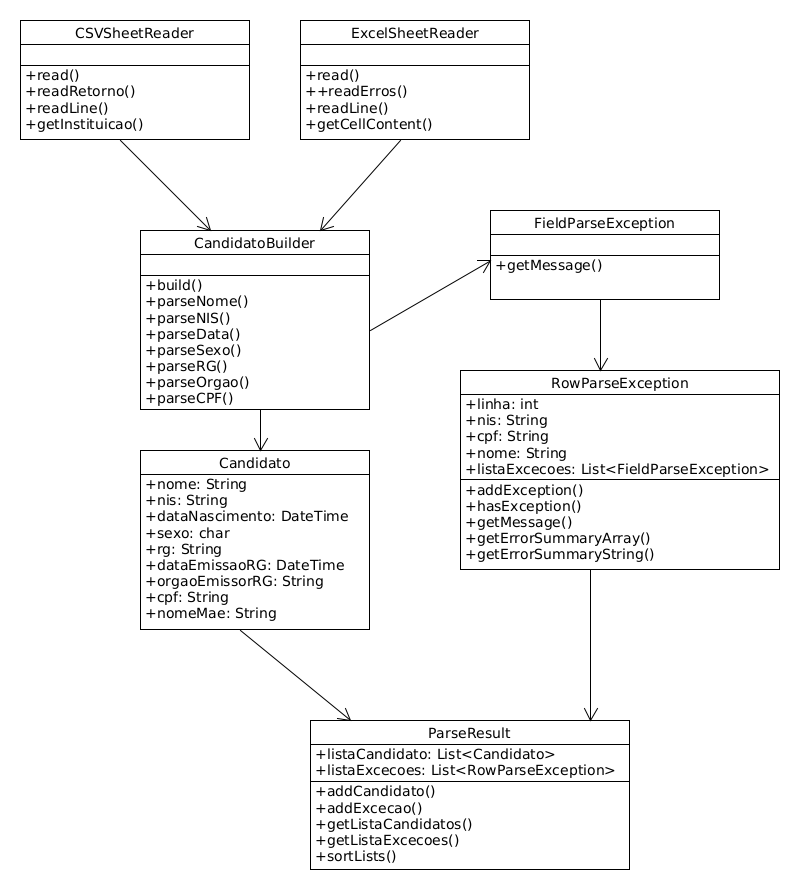
\includegraphics[scale=0.6]{img/envio-uml}
						
					\end{center}
				\end{figure}
	
				Em resumo, os dados dos candidatos solicitantes são extraídos de acordo com o tipo de arquivo de origem, pelas classes \textit{CSVSheetReader} e \textit{ExcelSheetReader} que, por sua vez, chamam a classe \textit{CandidatoBuilder} para validar os dados extraídos e, caso sejam 100\% válidos, um novo objeto \textit{Candidato} é gerado, do contrário, uma exceção do tipo \textit{RowParseException} é lançada com informações de todos os campos inválidos (por meio da classe \textit{FieldParseException}). Por fim, os dados são concentrados no objeto \textit{ParseResult} e estão prontos para exportação.
	
			\subsection{Interface Gráfica do Módulo de Envio}
	
				Como premissas no desenvolvimento do \textit{frontend} do \textit{IsenSys}, simplicidade e usabilidade sobressaem-se, mas sem perder a essência de uma aplicação robusta e consolidada. Na figura a seguir, está ilustrada a única tela do módulo de envio.
	
				\begin{figure}[ht]
					\begin{center}
						
						\caption{Tela do Módulo de Envio}
						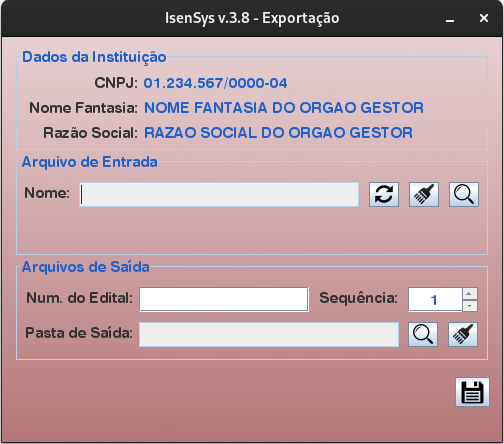
\includegraphics[scale=0.6]{img/envio-ui}
						
					\end{center}
				\end{figure}
	
				No painel 'Dados da Instituição', estão dispostas algumas informações exigidas no cabeçalho do arquivo de envio ao SISTAC, tais como CNPJ, nome fantasia e razão social do órgão gestor.
	
				No painel 'Arquivo de Entrada' é possível selecionar o arquivo de origem dos dados de solicitações dos candidatos, atualmente planilhas do \textit{Microsoft Excel} e arquivos \textit{csv} são suportados. Também é possível recarregar o arquivo previamente selecionado ou limpar sua seleção. Se um arquivo válido foi selecionado, algumas informações sobre o carregamento são mostradas na porção inferior deste painel, como ilustra a figura a seguir.
	
				\begin{figure}[ht]
					\begin{center}
						
						\caption{Tela do Módulo de Envio (arquivo carregado)}
						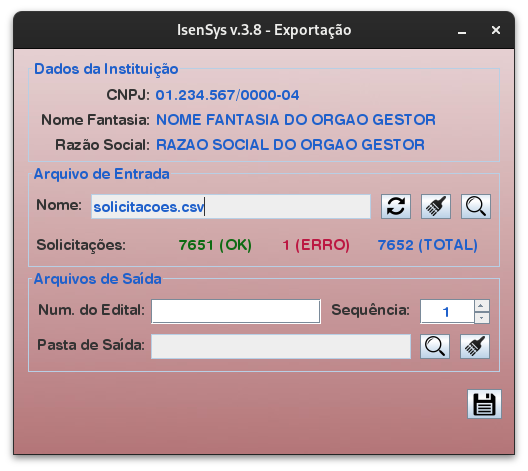
\includegraphics[scale=0.5]{img/envio-ui-loaded}
						
					\end{center}
				\end{figure}
	
				Os dois primeiros campos do painel 'Arquivos de Saída' (Num. do Edital e Sequência) também são exigências descritas no manual de envio do SISTAC \cite{sistac-formatos}. O campo 'Num. do Edital' faz parte do nome do arquivo de envio, juntamente com a identificação de sua sequência. Cada arquivo possui uma sequência geralmente iniciada em '1'. Se dois arquivos são gerados, temos então as sequências '1' e '2'. Sequências são reiniciadas a cada novo dia. Ainda neste painel, podemos escolher o diretório de escrita dos arquivos ou limpar sua seleção.

				Por fim, após todos os dados serem fornecidos na tela, a exportação pode ser realizada clicando no ícone de salvar (disquete). As figuras a seguir ilustram a saída dos arquivos após alimentar a tela com algumas informações.

				\clearpage
				\begin{figure}[ht]
					\begin{center}
						
						\caption{Tela do Módulo de Envio (preenchida) + Arquivos de Saída}
						
						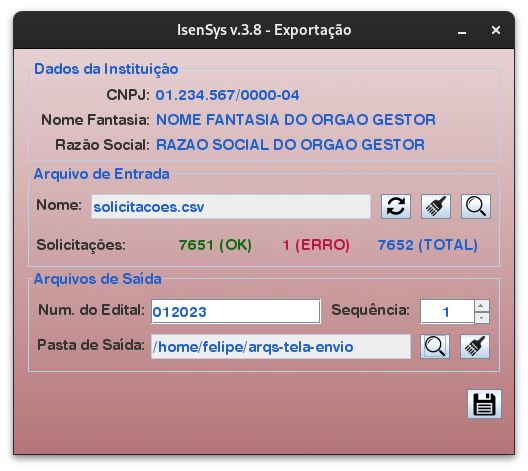
\includegraphics[scale=0.4]{img/envio-ui-processed}
						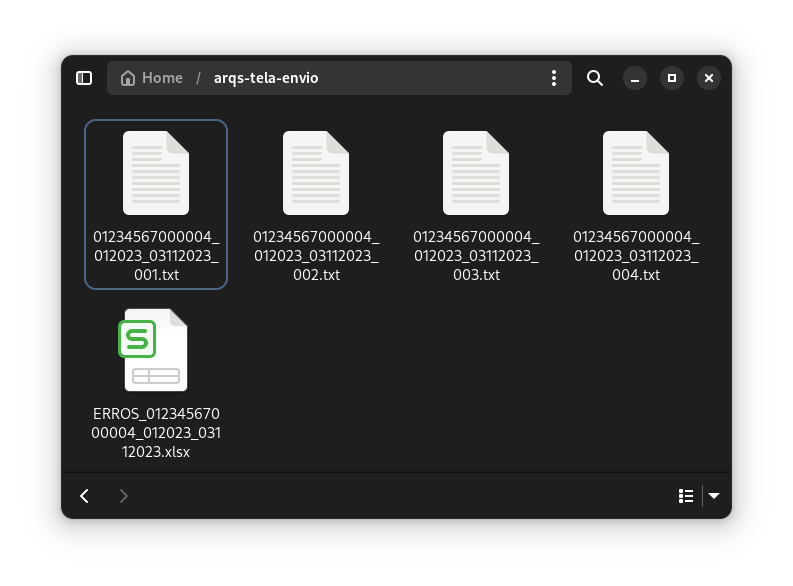
\includegraphics[scale=0.3]{img/envio-files}
						
					\end{center}
				\end{figure}

				De posse dos arquivos exportados, o envio já pode ser realizado à plataforma do SISTAC. A planilha gerada pode ser consultada de forma avulsa, mas é recomendável mantê-la inalterada, pois é necessária para a montagem dos relatórios de publicação nos módulos de retorno.

		\section{Desenvolvimento dos Módulos de Retorno}
	
			Esta seção tem por objetivo detalhar o desenvolvimento do \textit{backend} de processamento do(s) arquivo(s) de retorno do SISTAC. A partir dele(s) é possível gerar relatórios com resultados e algumas métricas e estatísticas úteis ao órgão gestor, todos prontos para publicação.
	
			Utilizando a mesma metodologia abordada na seção anterior, vamos começar compreendendo o fluxo de informações, conhecendo as classes envolvidas no processo e, posteriormente, a interface gráfica.
	
			\subsection{Modelagem de um Retorno}
	
				Para estes módulos, apenas alguns dados das solicitações dos candidatos são aproveitados. Temos então a concepção da classe \textit{Retorno}, de acordo com a especificação descrita na figura a seguir:
	
				% Tabela gerada com o auxílio da aplicação: https://www.tablesgenerator.com/latex_tables
				\begin{figure}[ht]
					\begin{center}
						
						\caption{Modelagem da Entidade \textit{Retorno}}
							
						\begin{tabular}{|l|}
							\hline
							\multicolumn{1}{|c|}{\textbf{Retorno}} \\ \hline
							+situacao: char                        \\
							+nome: String                          \\
							+nis: String                           \\
							+cpf: String                           \\
							+motivo: int                           \\
							+nomeAnterior: String                  \\ \hline
							+defere()                              \\
							+isDeferido()                          \\
							+compareTo()                           \\ \hline
						\end{tabular}
						
					\end{center}
				\end{figure}
	
			\subsection{A classe \textit{ListaRetornos}}

				Esta classe concentra todos os \textit{Retorno}'s extraídos do arquivo de retorno do SISTAC, com adição dos atributos do órgão gestor e dados do edital de publicação. Será detalhado ao decorrer desta monografia os dois módulos de retorno, que são: retorno preliminar [\ref{retorno-preliminar}] e retorno definitivo [\ref{retorno-definitivo}]. Por enquanto, temos que esta classe armazena dados úteis aos dois módulos.

				% Tabela gerada com o auxílio da aplicação: https://www.tablesgenerator.com/latex_tables
				\begin{figure}[ht]
					\begin{center}
						
						\caption{Diagrama de classe de \textit{ListaRetornos}}
						
						\begin{tabular}{|l|}
							\hline
							\multicolumn{1}{|c|}{\textbf{ListaRetornos}}         \\ \hline
							+listaRetornos: List\textless{}Retorno\textgreater{} \\
							+cnpj: String                                        \\
							+nomeFantasia: String                                \\
							+razaoSocial: String                                 \\
							+edital: String                                      \\
							+dataEdital: String                                  \\
							+cabecalho: String                                   \\ \hline
							+get()                                               \\
							+size()                                              \\
							+getList()                                           \\
							+clone()                                             \\
							+add()                                               \\
							+update()                                            \\
							+sort()                                              \\ \hline
						\end{tabular}
						
					\end{center}
				\end{figure}
	
			\subsection{A classe \textit{Compilacao}} \label{compilacao}
	
				Esta classe possui a incumbência de gravar ou carregar um arquivo com a extensão \textit{(.icf - IsenSys Compilation File)} objetos da classe \textit{ListaRetornos}, útil no processamento do retorno definitivo. Eis o seu diagrama de classe:
	
				% Tabela gerada com o auxílio da aplicação: https://www.tablesgenerator.com/latex_tables
				\begin{figure}[ht]
					\begin{center}
						
						\caption{Diagrama de Classe de \textit{Compilacao}}
						
						\begin{tabular}{|l|}
						\hline
						\multicolumn{1}{|c|}{\textbf{Compilacao}} \\ \hline
						\\ \hline
						+save()                                    \\
						+load()                                    \\ \hline
						\end{tabular}
						
					\end{center}
				\end{figure}
	
			\subsection{Modelagem de uma Situacao} \label{situacao}
	
				De acordo com o manual do SISTAC \cite{sistac-formatos}, existem algumas situações de indeferimento definidas. No \textit{IsenSys}, tais situações são armazenadas em um arquivo (\textit{csv}) com codificação UTF-8 no diretório de recursos do sistema [\ref{recursos}]. Durante a confecção dos editais de publicação, as situações são carregadas do arquivo e enviadas à classe geradora de relatórios, juntamente com os dados dos retornos.
	
				% Tabela gerada com o auxílio da aplicação: https://www.tablesgenerator.com/latex_tables
				\begin{figure}[ht]
					\begin{center}
						
						\caption{Modelagem da Entidade \textit{Situacao}}
						
						\begin{tabular}{|l|}
							\hline
							\multicolumn{1}{|c|}{\textbf{Situacao}} \\ \hline
							+id: String                             \\
							+motivo: String                         \\
							+descricao: String                      \\ \hline
							                                        \\ \hline
						\end{tabular}
						
					\end{center}
				\end{figure}
	
			\subsection{A classe \textit{SituacaoDAO}}
	
				Basicamente esta classe é responsável por carregar as situações a partir do arquivo \textit{'situacoes.csv'}, contido no diretório de recursos do \textit{IsenSys}, para uma lista de \textit{Situacao} [\ref{situacao}], útil na confecção dos relatórios de publicação.
	
				% Tabela gerada com o auxílio da aplicação: https://www.tablesgenerator.com/latex_tables
				\begin{figure}[ht]
					\begin{center}
						
						\caption{Diagrama de Classe de \textit{SituacaoDAO}}
						
						\begin{tabular}{|l|}
							\hline
							\multicolumn{1}{|c|}{\textbf{SituacaoDAO}} \\ \hline
							                                           \\ \hline
							+load()                                    \\ \hline
						\end{tabular}
						
					\end{center}
				\end{figure}
	
			\subsection{Geradores de Relatório}
	
				O \textit{IsenSys} implementa três tipos de relatórios a partir dos dados provenientes do(s) arquivo(s) de retorno do SISTAC. Cada uma das classes que os implementam contam com o método '\textit{export()}', que é capaz de compilar e exportar o relatório para o formato PDF. A figura a seguir ilustra as estruturas de classe dos três geradores.
	
				% Tabela gerada com o auxílio da aplicação: https://www.tablesgenerator.com/latex_tables
				\begin{figure}[ht]
					\begin{center}
						
						\caption{Diagramas de Classe dos Geradores de Relatório}
						
						\begin{tabular}{|l|l|l|l|l|}
						\cline{1-1} \cline{3-3} \cline{5-5}
						\multicolumn{1}{|c|}{\textbf{PDFEstatisticas}} &  & \multicolumn{1}{c|}{\textbf{PDFResultado}} &  & \multicolumn{1}{c|}{\textbf{PDFSimilaridade}} \\ \cline{1-1} \cline{3-3} \cline{5-5} 
						&  &                                          &  &                                               \\ \cline{1-1} \cline{3-3} \cline{5-5} 
						+export()                                &  & +export()                                &  & +export()                                     \\ \cline{1-1} \cline{3-3} \cline{5-5} 
						\end{tabular}
						
					\end{center}
				\end{figure}
	
			\subsection{Integração dos Módulos de Retorno}
	
				Conhecendo individualmente os agentes envolvidos no módulo de retorno, podemos realizar uma abordagem integrada dos dois tipos de retorno: retorno preliminar e retorno definitivo.
	
				\subsubsection{Retorno Preliminar} \label{retorno-preliminar}
	
					Este é o módulo destinado ao processamento do resultado preliminar das solicitações de isenção. A figura a seguir ilustra o fluxo das informações através do módulo.
	
					\clearpage
					\begin{figure}[ht]
						\begin{center}
							
							\caption{Diagrama do Fluxo de Dados no Retorno Preliminar}
							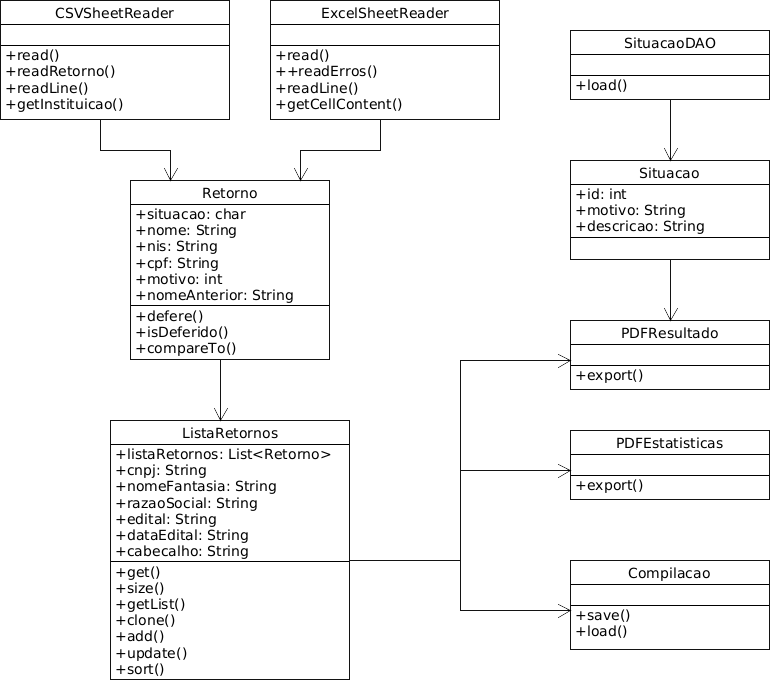
\includegraphics[scale=0.5]{img/retorno-prelim-uml}
							
						\end{center}
					\end{figure}
	
					Começando pelos arquivos de entrada, as classes \textit{CSVSheetReader} e \textit{ExcelSheetReader} carregam o(s) arquivo(s) de retorno do SISTAC e planilha de erros, respectivamente, produzindo então objetos da classe \textit{Retorno} que são agrupados em uma lista na classe \textit{ListaRetornos}.
	
					Na exportação, os dados armazenados na classe \textit{ListaRetornos} são enviados aos geradores de PDF implementados em \textit{PDFEstatisticas} e \textit{PDFResultado} e, por fim, salvos em um arquivo binário denominado de 'compilação', por meio da classe \textit{Compilacao}.
	
				\subsubsection{Tela do Módulo de Retorno Preliminar}
	
					A figura a seguir ilustra a implementação da interface gráfica do módulo de retorno preliminar do \textit{IsenSys}.
	
					\clearpage
					\begin{figure}[ht]
						\begin{center}
							
							\caption{Tela do Módulo de Retorno Preliminar}
							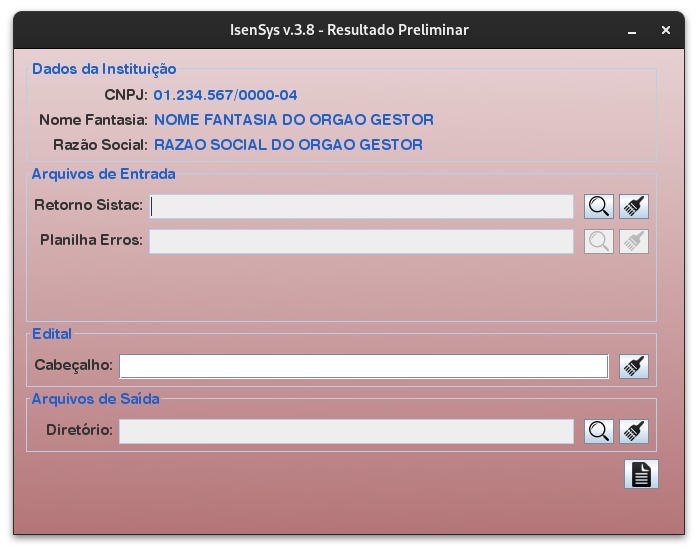
\includegraphics[scale=0.6]{img/retorno-prelim-ui}
							
						\end{center}
					\end{figure}
	
					No painel 'Dados da Instituição', estão dispostas algumas informações exigidas no cabeçalho do arquivo de envio ao SISTAC \cite{sistac-formatos}, tais como CNPJ, nome fantasia e razão social do órgão gestor.
	
					Em 'Arquivos de Entrada' é possível selecionar o(s) arquivo(s) de retorno do SISTAC e a planilha contendo os erros de validação (gerada no módulo de envio). O usuário também é capaz de limpar a seleção do(s) arquivo(s). A seguir estão enumerados alguns detalhes sobre os arquivos:
	
					\begin{itemize}
						
						\item \textbf{Retorno Sistac:} o usuário deve selecionar SEMPRE o primeiro arquivo de retorno do SISTAC, caso haja mais de um, o carregamento dos demais arquivos é feito de forma automática, basta que estejam no mesmo diretório do primeiro arquivo;
						\item \textbf{Planilha Erros:} aqui o usuário deve selecionar a planilha de erros gerada pelo módulo de envio do \textit{IsenSys};
						
					\end{itemize}
		
					Se um arquivo válido foi selecionado, algumas informações sobre o carregamento são mostradas na porção inferior deste painel, como ilustra a figura a seguir.
		
					\begin{figure}[ht]
						\begin{center}
							
							\caption{Tela do Módulo de Retorno Preliminar (preenchida)}
							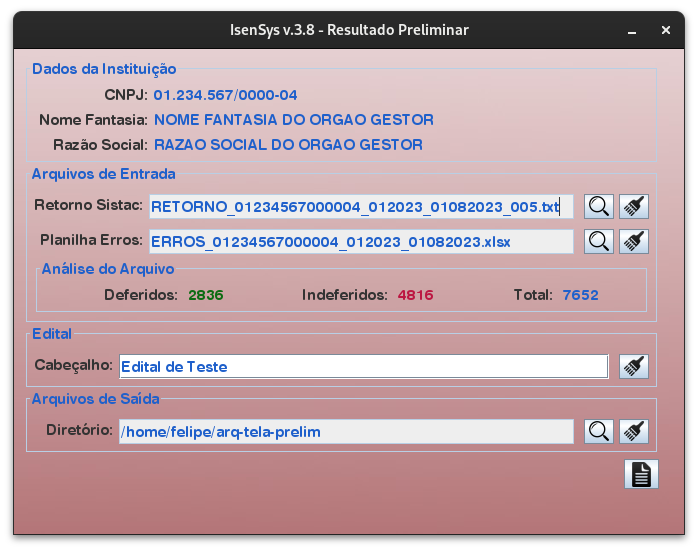
\includegraphics[scale=0.45]{img/retorno-prelim-ui-processed}
							
						\end{center}
					\end{figure}
		
					O nome do edital pode ser informado no campo de texto do painel 'Edital' e no painel 'Arquivos de Saída' é possível selecionar o diretório para saída dos arquivos gerados pelo módulo (resultados, relatório de estatísticas e arquivo de compilação), como mostra a figura a seguir.
		
					\begin{figure}[!ht]
						\begin{center}
							
							\caption{Arquivos de Saída do Módulo de Retorno Preliminar}
							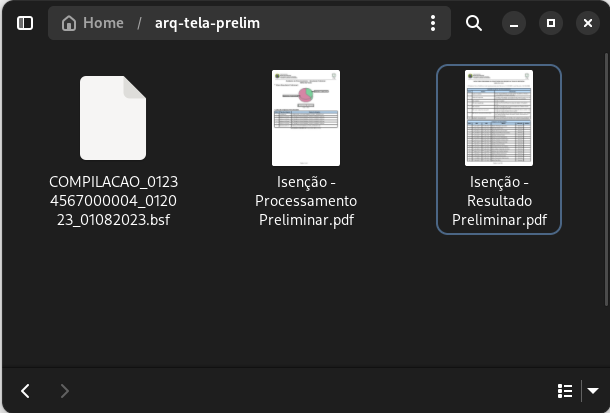
\includegraphics[scale=0.45]{img/retorno-prelim-files}
							
						\end{center}
					\end{figure}
		
				\subsubsection{Retorno Definitivo} \label{retorno-definitivo}
	
					Este é o módulo destinado ao processamento do resultado definitivo. É capaz de recuperar as informações do módulo de retorno preliminar, através de um arquivo de compilação (gerado pela classe \textit{Compilacao} [\ref{compilacao}]) e importar o(s) novo(s) arquivo(s) de retorno do SISTAC.

					\begin{figure}[ht]
						\begin{center}
							
							\caption{Diagrama do Fluxo de Dados no Retorno Definitivo}
							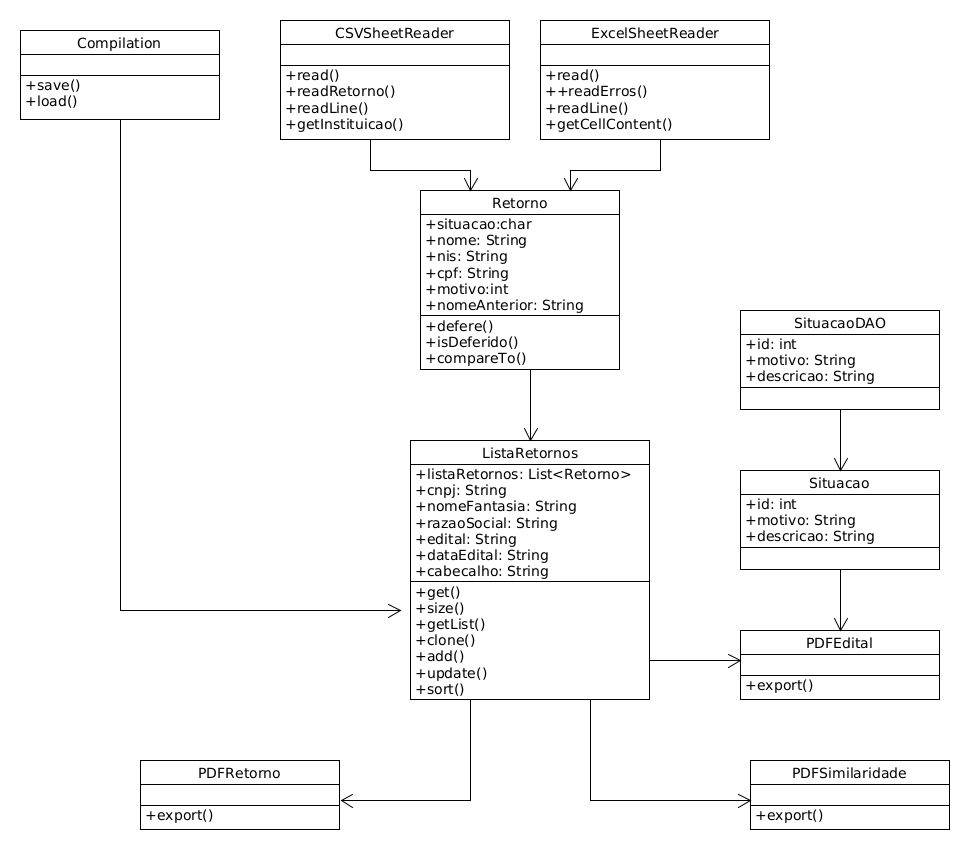
\includegraphics[scale=0.5]{img/retorno-def-uml}
							
						\end{center}
					\end{figure}
	
					Para o processamento do retorno definitivo, a principal classe alimentadora é a \textit{Compilacao} [\ref{compilacao}] que carrega os dados provenientes do módulo de resultado preliminar e, a princípio, já estão prontos para serem exportados como resultado definitivo.
	
				\subsubsection{Tela do Módulo de Retorno Definitivo}
	
					A figura a seguir ilustra a implementação da interface gráfica do módulo de retorno definitivo do \textit{IsenSys}.
	
					\begin{figure}[ht]
						\begin{center}
							
							\caption{Tela do Módulo de Retorno Definitivo}
							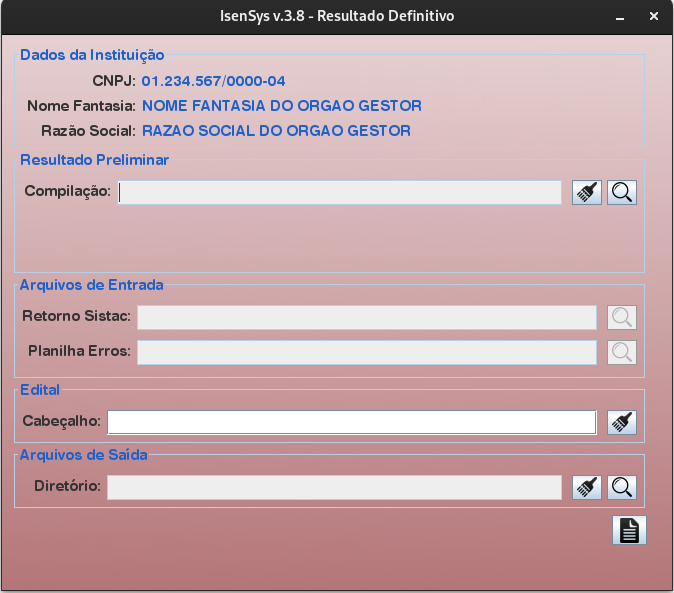
\includegraphics[scale=0.45]{img/retorno-def-ui}
							
						\end{center}
					\end{figure}
	
					Ao carregar o arquivo de compilação, algumas informações são exibidas na porção inferior do painel 'Resultado Preliminar'. O cabeçalho do edital também é carregado.
	
					Da mesma forma que no módulo do resultado preliminar, o arquivo de retorno a ser selecionado deve ser sempre o primeiro, os demais são carregados automaticamente desde que estejam no mesmo diretório do primeiro arquivo.
	
					Se algum arquivo de entrada for selecionado, tanto de retorno quanto de erros, os dados são mesclados com os provenientes do resultado preliminar da seguinte forma:
	
					\begin{itemize}
						
						\item \textbf{Retorno Sistac:} se o candidato retornado tiver sua solicitação \textbf{indeferida}, apenas seu status é atualizado na lista preexistente. Caso tenha sido \textbf{deferida}, além de ter seu estado alterado, o novo deferido fará parte de uma nova lista, para futuro cálculo de similaridade [\ref{similaridade}];
						
						\item \textbf{Erros:} aqui todos os erros são mesclados.
						
					\end{itemize}

		\section{Relatório de Similaridade} \label{similaridade}
		
			Uma necessidade especial tornou necessária a implementação de um relatório que calculasse o quão similar é o nome de um candidato na fase de solicitação (1{\textordfeminine} instância) e na fase de recurso (2{\textordfeminine} instância).
			
			Empiricamente foi detectado que um candidato qualquer que teve sua solicitação de isenção indeferida em primeira instância e recursou trocando seus dados pessoais pelos de alguém que tem ciência de isenção garantida, teve recurso deferido pelo SISTAC.
			
			Como forma de evitar que tais candidatos praticantes deste ato ilícito tivessem isenção deferida sem ciência do órgão gestor, foi desenvolvido um relatório chamado de 'Relatório de Similaridade e Distância entre Nomes', que computa porcentagens das referidas métricas utilizando o algoritmo de \textit{Jaro-Winkler} [\ref{jaro-winkler}], entre o nome informado na fase de solicitação e recurso, pelo candidato.
			
			O algoritmo é executado tomando como base candidatos que tiveram solicitação de isenção indeferida em primeira instância, mas deferida após recurso, gerando um relatório com o comparativo entre nomes e as duas métricas (similaridade e distância), ordenado pela ordem crescente de similaridade.
			
			Algumas classes estão envolvidas na confecção deste relatório, são elas: \textit{Similaridade} e \textit{JaroWinkler}, além do gerador de PDF: \textit{PDFSimilaridade}.
			
			\subsection{Modelagem de uma Similaridade}
			
				Esta classe contém alguns atributos úteis para confecção do relatório de similaridade entre nomes. A figura a seguir ilustra seu diagrama de classe.
				
				% Tabela gerada com o auxílio da aplicação: https://www.tablesgenerator.com/latex_tables
				\begin{figure}[ht]
					\begin{center}
						
						\caption{Diagrama de Classe de uma Similaridade}
						
						\begin{tabular}{|l|}
							\hline
							\multicolumn{1}{|c|}{\textbf{Similaridade}} \\ \hline
							+nomeSolicitacao: String                    \\
							+nomeRecurso: String                        \\
							+distancia: double                          \\
							+similaridade: double                       \\ \hline
							\\ \hline
						\end{tabular}
						
					\end{center}
				\end{figure}

			\subsection{A classe \textit{JaroWinkler}}
			
				É uma classe auxiliar que computa o algoritmo de \textit{Jaro-Winkler} [\ref{jaro-winkler}] nos dados dos candidatos recursantes. Para cálculo das métricas de distância e similaridade, a biblioteca \textit{Apache Commons Text\texttrademark} [\ref{commons-text}] foi utilizada. A seguir seu diagrama de classe.
			
				% Tabela gerada com o auxílio da aplicação: https://www.tablesgenerator.com/latex_tables
				\begin{figure}[ht]
					\begin{center}
						
						\caption{Diagrama de Classe de \textit{JaroWinkler}}
						
						\begin{tabular}{|l|}
							\hline
							\multicolumn{1}{|c|}{\textbf{JaroWinkler}} \\ \hline
							\\ \hline
							+compute()                                \\ \hline
						\end{tabular}
						
					\end{center}
				\end{figure}

			\subsection{Montagem do Relatório de Similaridade}
			
				Realizando uma abordagem integrada, conhecendo os agentes envolvidos na produção do relatório, temos o seguinte diagrama.
				
				\begin{figure}[ht]
					\begin{center}
						
						\caption{Diagrama do Fluxo de Dados no Relatório}
						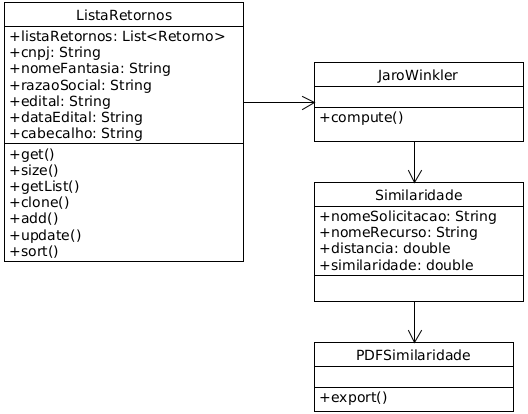
\includegraphics[scale=0.65]{img/jaro-winkler-uml}
						
					\end{center}
				\end{figure}
				
				De uma forma prática e funcional, os dados dos candidatos solicitantes, provenientes de \textit{ListaRetornos}, são encaminhados à classe \textit{JaroWinkler} para computação das métricas de distância e similaridade e salvamento em objetos da classe \textit{Similaridade}. Por fim, \textit{PDFSimilaridade} aproveita estes dados para a confecção do relatório.

		\section{Diretório de Recursos do \textit{IsenSys}} \label{recursos}
		
			O \textit{IsenSys} conta com alguns arquivos de configuração e recursos que estão dispostos em um diretório chamado '\textit{res}', existente no mesmo nível de diretório do arquivo executável do \textit{IsenSys}.
			
			A seguir estão listados os recursos e seus caminhos relativos ao diretório raiz da aplicação.
			
			\begin{itemize}
				
				\item \textbf{\textit{config/program.dat:}} contém as configurações globais do sistema;
				\item \textbf{\textit{fonts/fonts-extension.jar:}} fontes utilizadas na confecção dos relatórios;
				\item \textbf{\textit{i18n/*.lng:}} arquivos contendo as \textit{strings} de interface do sistema;
				\item \textbf{\textit{icon/*.png:}} contém os ícones utilizados nas telas;
				\item \textbf{\textit{img/:}} diretório contendo as imagens de fundo das telas;
				\item \textbf{\textit{relatorios/*.jasper:}} arquivos-modelos dos relatórios;
				\item \textbf{\textit{situacoes/situacoes.csv:}} arquivo contendo as situações de indeferimento.
				
			\end{itemize}
			
			Para o correto funcionamento do sistema é recomendável que o usuário não altere o conteúdo destes arquivos manualmente, tampouco os exclua, renomeie ou os troque de diretório.

	\chapter{Implementação e Resultados}
	
		A versão corrente do sistema (v.3.8) foi implementada no início de Junho de 2023 na COMPEC, com o objetivo de ter como piloto o processamento das solicitações de isenção do Processo Seletivo Contínuo - PSC 2024 - Etapas 1 e 2, fruto dos Editais de n{\textordmasculine} \cite{edital-13} e \cite{edital-14}/GR/UFAM.
		
		Por pura coincidência, o PSC 2024 é a primeira edição a possuir a modalidade de isenção via CadÚnico logo nas primeiras etapas do processo, opção que só era concedida aos candidatos da 3{\textordfeminine} etapa.
		
		Segundo os editais que regem o processo seletivo, o período de solicitações de isenção de taxa de inscrição foi entre as 10h do dia 01/06/2023 até as 17h do dia seguinte, onde foram recebidas \textbf{7.652 solicitações na 1{\textordfeminine} etapa} e \textbf{3.052 na 2{\textordfeminine} etapa}, totalizando incríveis \textbf{10.704 solicitações}.
		
		A computação das solicitações foi realizada em um computador da marca Lenovo, modelo M93p com as seguintes especificações:
		
		\begin{itemize}
			
			\item Memória RAM DDR3-1600, com capacidade total de 16GB;
			\item Processador Intel{\textregistered} Core{\texttrademark} i5-4570 de 3.60 GHz;
			\item Sistema operacional Arch Linux de 64 bits, com \textit{engine} gráfica GNOME;
			\item Monitor padrão da marca HP, modelo V225hz, com resolução de 1920x1080.
			
		\end{itemize}
		
		Seguindo o fluxo padrão do processo de isenção, começamos pela preparação de dados para envio ao SISTAC, através da Tela de Envio. Toda a interação com a interface gráfica se mostrou estável e não foi detectado nenhum erro de execução ou travamentos, mesmo com alto volume de dados.
		
		% Tabela gerada com o auxílio da aplicação: https://www.tablesgenerator.com/latex_tables
		\begin{table}[ht]
			\begin{center}
				
				\caption{Tempos de Processamento de Dados [Preliminar]}
				
				\begin{tabular}{|c|c|c|c|}
						\hline
						\textbf{Etapa} & \textbf{\begin{tabular}[c]{@{}c@{}}Qtd. de\\ Solicitações\end{tabular}} & \textbf{\begin{tabular}[c]{@{}c@{}}Tempo de\\ Execução (ms)\end{tabular}} & \textbf{\begin{tabular}[c]{@{}c@{}}Tempo de\\ Exportação de\\ Relatórios (s)\end{tabular}} \\ \hline
						1              & 7.652                                                                   & 1.500                                                                     & 2.7                                                                                        \\ \hline
						2              & 3.052                                                                   & 780                                                                       & 1.25                                                                                       \\ \hline
				\end{tabular}
			\end{center}
		\end{table}
		
		% Tabela gerada com o auxílio da aplicação: https://www.tablesgenerator.com/latex_tables
		\begin{table}[ht]
			\begin{center}
				
				\caption{Tempos de Processamento de Dados [Definitivo]}
				
				\begin{tabular}{|c|c|c|c|}
					\hline
					\textbf{Etapa} & \textbf{\begin{tabular}[c]{@{}c@{}}Qtd. de\\ Recursos\end{tabular}} & \textbf{\begin{tabular}[c]{@{}c@{}}Tempo de\\ Execução (ms)\end{tabular}} & \textbf{\begin{tabular}[c]{@{}c@{}}Tempo de\\ Exportação de\\ Relatórios (s)\end{tabular}} \\ \hline
					1              & 357                                                                     & 250                                                                       & 3.1                                                                                        \\ \hline
					2              & 157                                                                     & 138                                                                       & 2.07                                                                                       \\ \hline
				\end{tabular}
			\end{center}
		\end{table}
		
		Como ilustrado em números, o \textit{IsenSys} conseguiu reduzir drasticamente o tempo de processamento das solicitações, processo realizado por humanos antes da implementação do sistema. Antes havia uma equipe que, de posse dos dados de solicitação, realizavam a confecção dos arquivos de envio ao SISTAC de forma artesanal, processo lento que se estendia por dias e era extremamente suscetível a erros.
		
		Além da confecção manual dos arquivos \textit{csv}, perdia-se muito tempo no processo de envio de lotes ao SISTAC pois, ao detectar o primeiro erro de preenchimento de arquivo, cancela todo o envio do lote e sinaliza apenas o erro corrente. Logo, corrigia-se manualmente o erro e uma nova submissão era realizada, até que o lote fosse totalmente recebido, sem erros.
		
		Em concursos com maior volume de solicitações estima-se que pelo menos 25 a 30 tentativas de envio eram realizadas à plataforma. É muito provável que esta realidade estenda-se em mais órgãos do Poder Executivo utilizadores do SISTAC e é quando o \textit{IsenSys} pode servir como aplicação institucionalizada, visando eficiência e colaboração no serviço público.
		
		A otimização implementada no \textit{IsenSys} faz com que os dados das solicitações passem por filtros analistas de dados, implementados de acordo com as normativas do manual do SISTAC \cite{sistac-formatos}. Ao detectar alguma disparidade entre o dado e o formato aceito, o \textit{IsenSys} tenta ajustá-lo e caso não seja possível, o separa em uma lista de erros e o processamento continua.
		
		Ao fim do processo, um arquivo de envio 100\% válido no formato do SISTAC é gerado e os erros, separados em uma planilha, para futura confecção dos relatórios de resultados preliminar e definitivo.
		
		O diagrama a seguir ilustra o pré-processamento de dados realizado tanto pelo SISTAC quanto pelo \textit{IsenSys}. Podemos verificar que, ao primeiro erro encontrado no arquivo de solicitações, o SISTAC rejeita o lote por completo.
		
		\begin{figure}[ht]
			\begin{center}
				
				\caption{Diagrama Comparativo entre o SISTAC e IsenSys}
				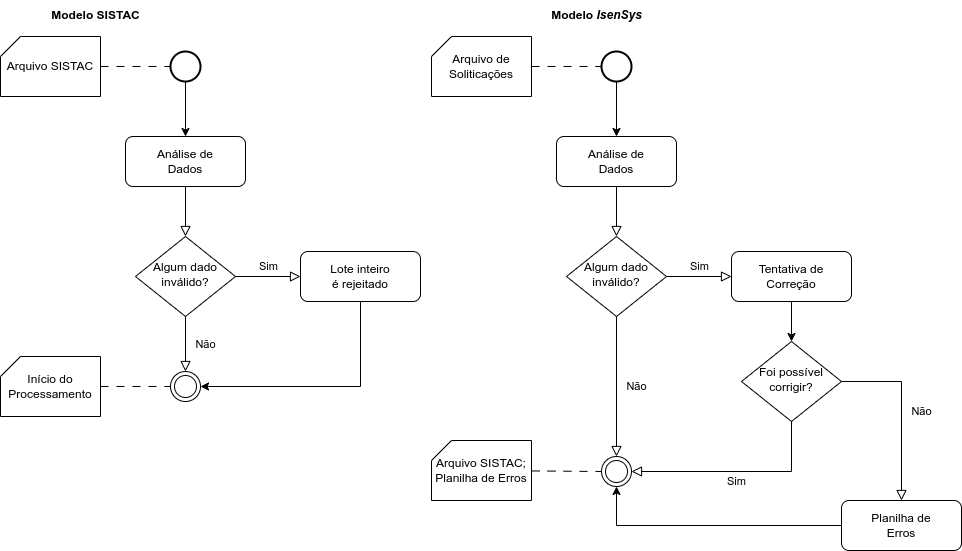
\includegraphics[scale=0.4]{img/diagrama-ativs-ganhos}
				
			\end{center}
		\end{figure}
		
		Graças à implementação do \textit{IsenSys}, a COMPEC conseguiu reduzir os tempos de processamento de solicitações de isenção de dias para segundos. Atualmente, pouco tempo após o término do prazo de solicitação ou recurso, os resultados preliminares ou definitivos já podem ser confeccionados.
		
		A tabela a seguir traz um comparativo entre o tempo necessário para confeccionar um arquivo de envio válido ao SISTAC, utilizando o processo manual e o \textit{IsenSys}. Vale ressaltar que nos dois processos, apenas o \textit{IsenSys} foi utilizado, as quantidades de dias foram calculadas com base em concursos anteriores de porte semelhante realizados pela COMPEC, utilizando as mesmas metodologias.
		
		% Tabela gerada com o auxílio da aplicação: https://www.tablesgenerator.com/latex_tables
		\begin{table}[ht]
			\begin{center}
				
				\caption{Comparativo de Tempo de Processamento do Arquivo de Envio}
				
				\begin{tabular}{|l|c|c|c|}
					\hline
					\multicolumn{1}{|c|}{\textbf{Processo}} & \textbf{\begin{tabular}[c]{@{}c@{}}Qtd.\\ Solicitações\end{tabular}} & \textbf{\begin{tabular}[c]{@{}c@{}}Preparo\\ Manual (dias)\end{tabular}} & \textbf{\begin{tabular}[c]{@{}c@{}}Preparo no\\ IsenSys (s)\end{tabular}} \\ \hline
					PSC 2023                                & 11.477                                                               & 15                                                                        & 5                                                                           \\ \hline
					PSTEC 2023                              & 5.020                                                                & 13                                                                        & 4                                                                           \\ \hline
				\end{tabular}
			\end{center}
		\end{table}
		
		Vimos que, com a implementação do \textit{IsenSys}, foi possível reduzir custos com contratação temporária de pessoal e recursos como impressão em papel, tonner de impressora e energia elétrica, tornando o serviço eficiente e com resultado preciso com alguns cliques e em alguns segundos.

	\chapter{Conclusões}
	
		\section{Considerações Finais}
	
			Visando valores como agilidade, lisura e transparência no processamento das solicitações de isenção de taxa de inscrição na modalidade CadÚnico, o \textit{IsenSys} surgiu como agente concretizador destes anseios, possibilitando que um órgão gestor consiga preparar dados para envio ao SISTAC e, após seu processo de análise, gerar relatórios de publicação de resultados e relatórios com estatísticas e métricas.
			
			Os resultados obtidos foram de grande satisfação tanto pela COMPEC, quanto pela sociedade, que tiveram um retorno ágil e preciso, respeitando todos os requisitos dispostos nos editais do concurso piloto e instruções normativas sobre o processo de isenção, de acordo com os manuais do SISTAC.
			
			Pode-se afirmar então que o objetivo principal do \textit{IsenSys} foi atingido. A aplicação foi construída utilizando uma linguagem de programação amplamente aceita e suportada no mercado, respeitando as boas práticas de programação e convenções internacionais, mantendo sempre a organização e comentários no código-fonte de forma a facilitar futuras colaborações.
	
		\section{Limitações e Propostas de Atualizações}
		
			Não há nada que exista que não possa ser melhorado e, partindo desse pressuposto, algumas otimizações e adições de novos recursos já foram mapeadas durante o processo de desenvolvimento e que, devido ao curto tempo para implementação e conclusão desta monografia, ainda não puderam ser incorporados ao projeto. Listar-se-á algumas:
			
			\begin{itemize}
				
				\item Estender o suporte do \textit{IsenSys} à máquinas de 32-bits, com a utilização do JDK 8;
				\item Implementar layouts dinâmicos na interface gráfica, de forma a permitir o redimensionamento das janelas;
				\item Permitir que o número de edital contenha caracteres alfanuméricos de forma a abranger esta atualização recente do SISTAC;
				\item Adicionar interfaces gráficas para gerência dos recursos do sistema tais como logomarca e arquivo de situações;
				\item Utilizar banco de dados para salvar configurações;
				\item Integrar as outras modalidades de isenção de taxa de inscrição, como a modalidade de análise documental, definida pela Lei n{\textordmasculine} 12.799, de 10 de abril de 2013 \cite{lei-12799}, e doadores de medula óssea, regulamentado pela Lei n{\textordmasculine} 13.656, de 30 de abril de 2018 \cite{lei-13656}.
				
			\end{itemize}
			
			O código-fonte em sua íntegra está disponível no repositório GitHub sob os links:
			
			\begin{itemize}
				
				\item \textbf{IsenSys:} \url{https://github.com/icomp-felipe/java-compec-isensys}
				\item \textbf{Phills Libs (dependência):} \url{https://github.com/icomp-felipe/phills-libs}
				\item \textbf{Relatórios:} \url{https://github.com/icomp-felipe/jasper-compec-isensys}
				
			\end{itemize}

	% ----------| Elementos Pós-Textuais |----------
	\postextual
	\Spacing{1.5}

	% ----------| Referências Bibliográficas |----------
	\bibliography{monografia-felipe-andre-ft}

	% ----------| Anexos |----------
	\begin{anexosenv}
		
		\chapter{Resultado Definitivo da Isenção do PSC 2023 (apenas algumas páginas)}
		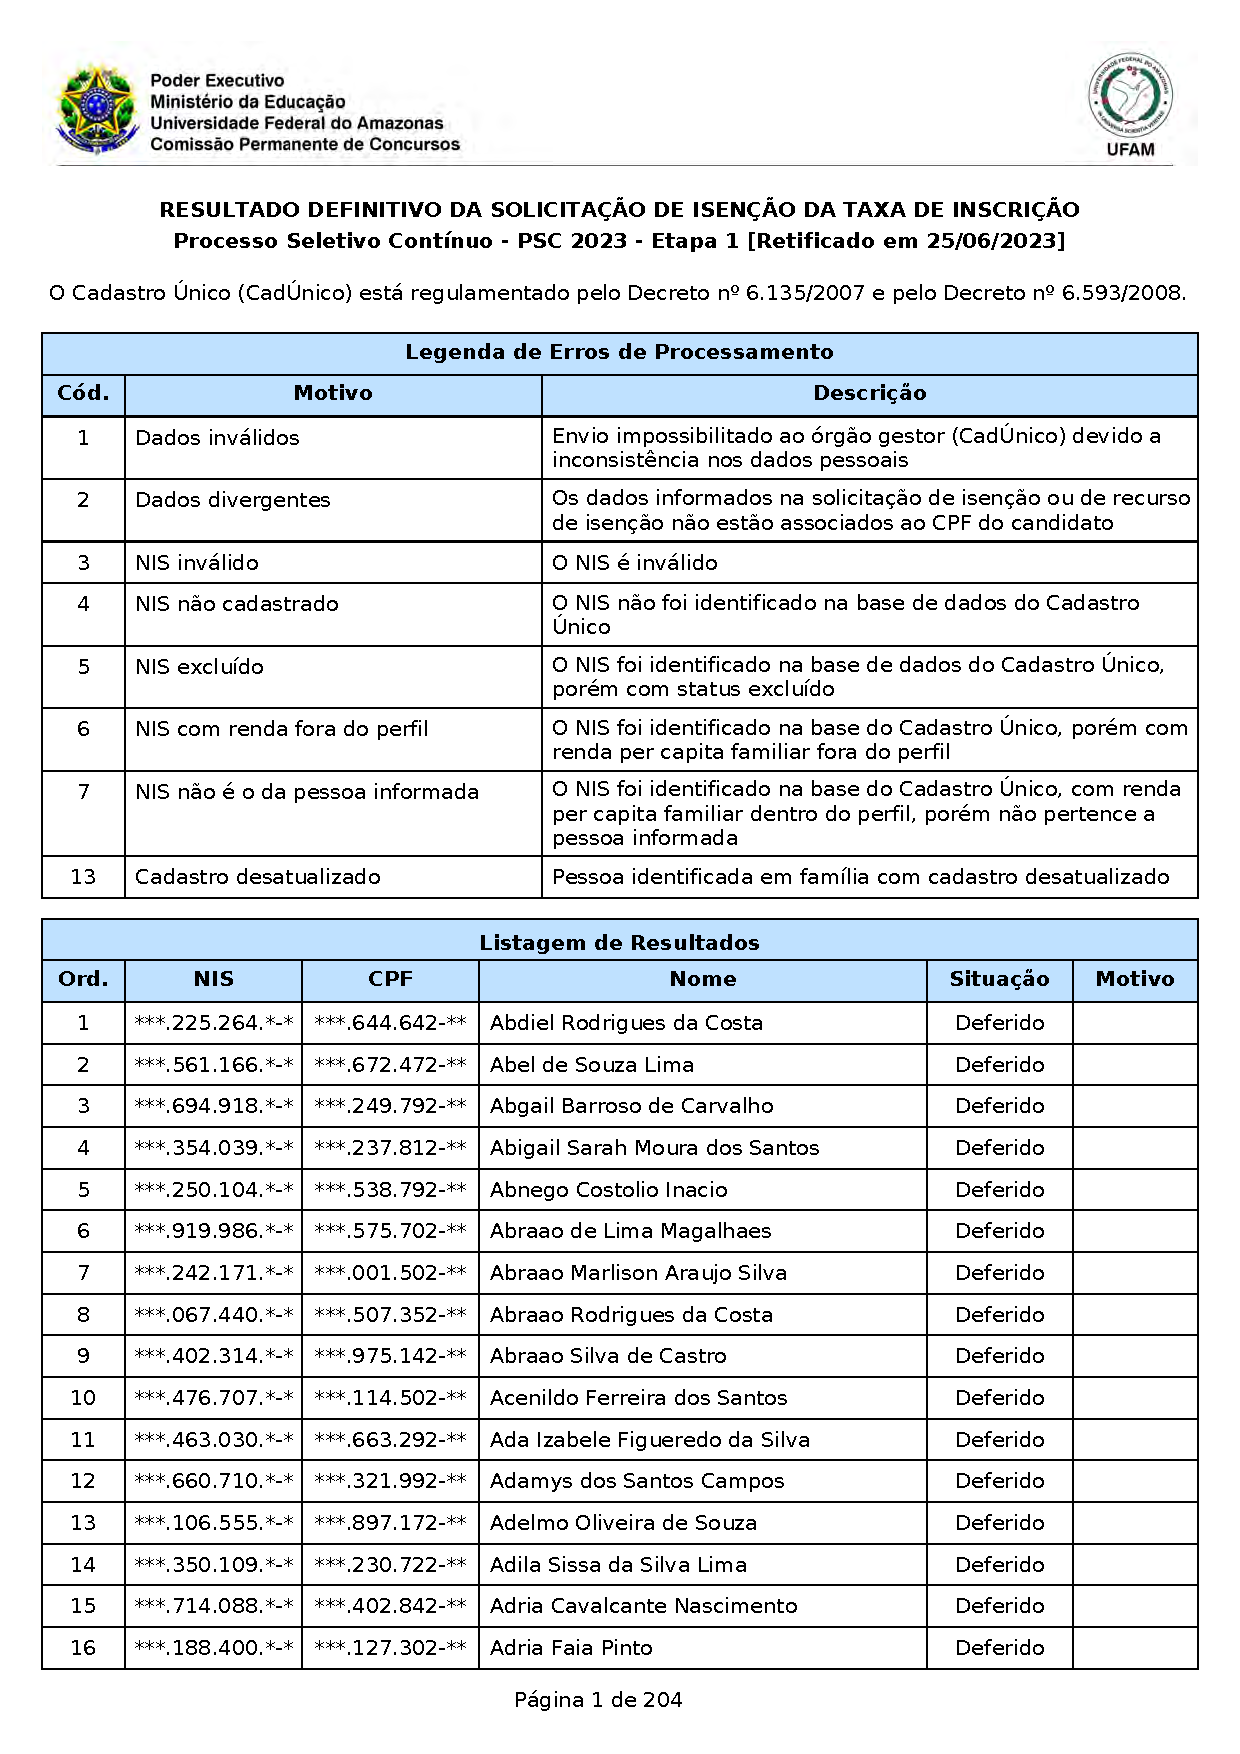
\includepdf[pages=-,pagecommand={},width=175 mm]{anexos/psc2023-e12-resultado-definitivo}
		
		\chapter{Relatório de Similaridade Aplicado no PSC 2023 (apenas algumas páginas)}
		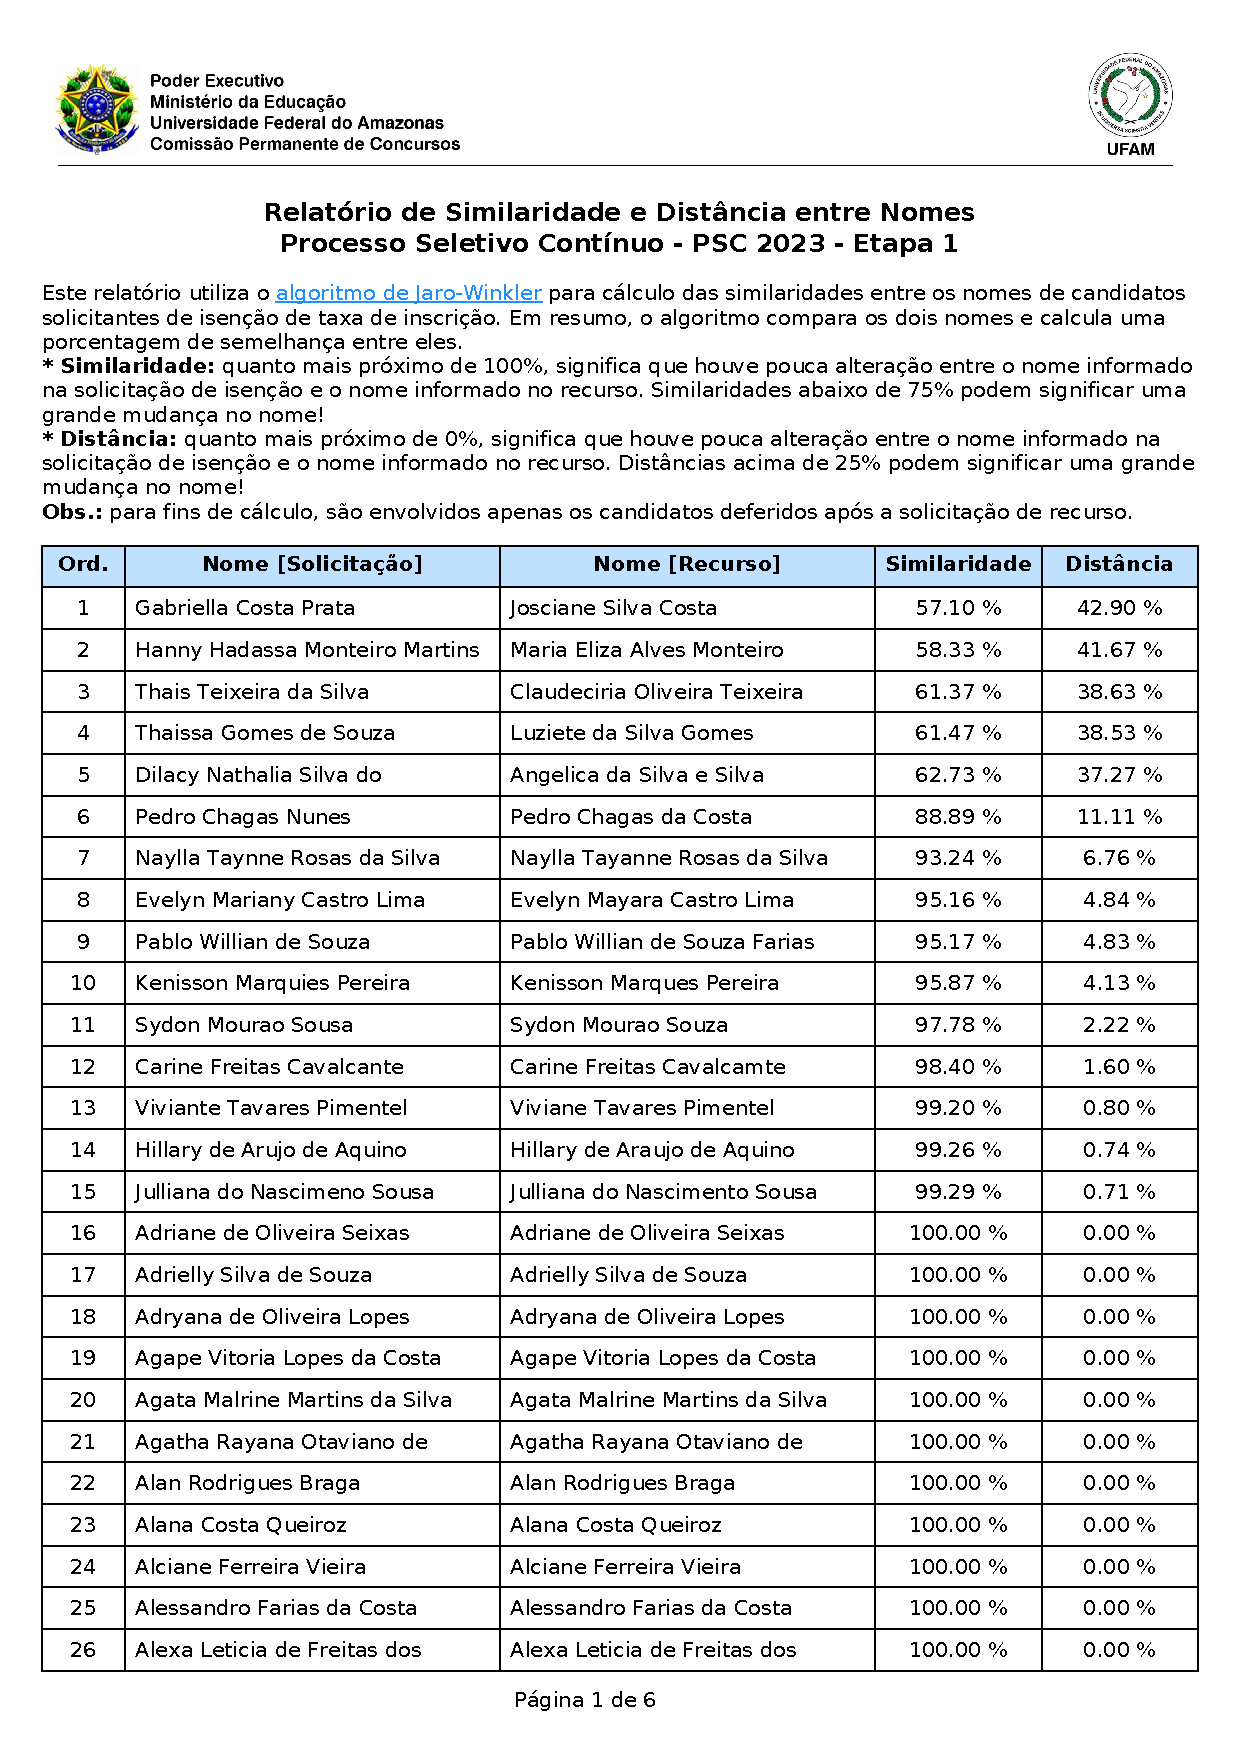
\includepdf[pages=-,pagecommand={},width=175 mm]{anexos/psc2023-e12-relatorio-similaridade}
		
		\chapter{Relatório de Estatísticas de Processamento (apenas algumas páginas)}
		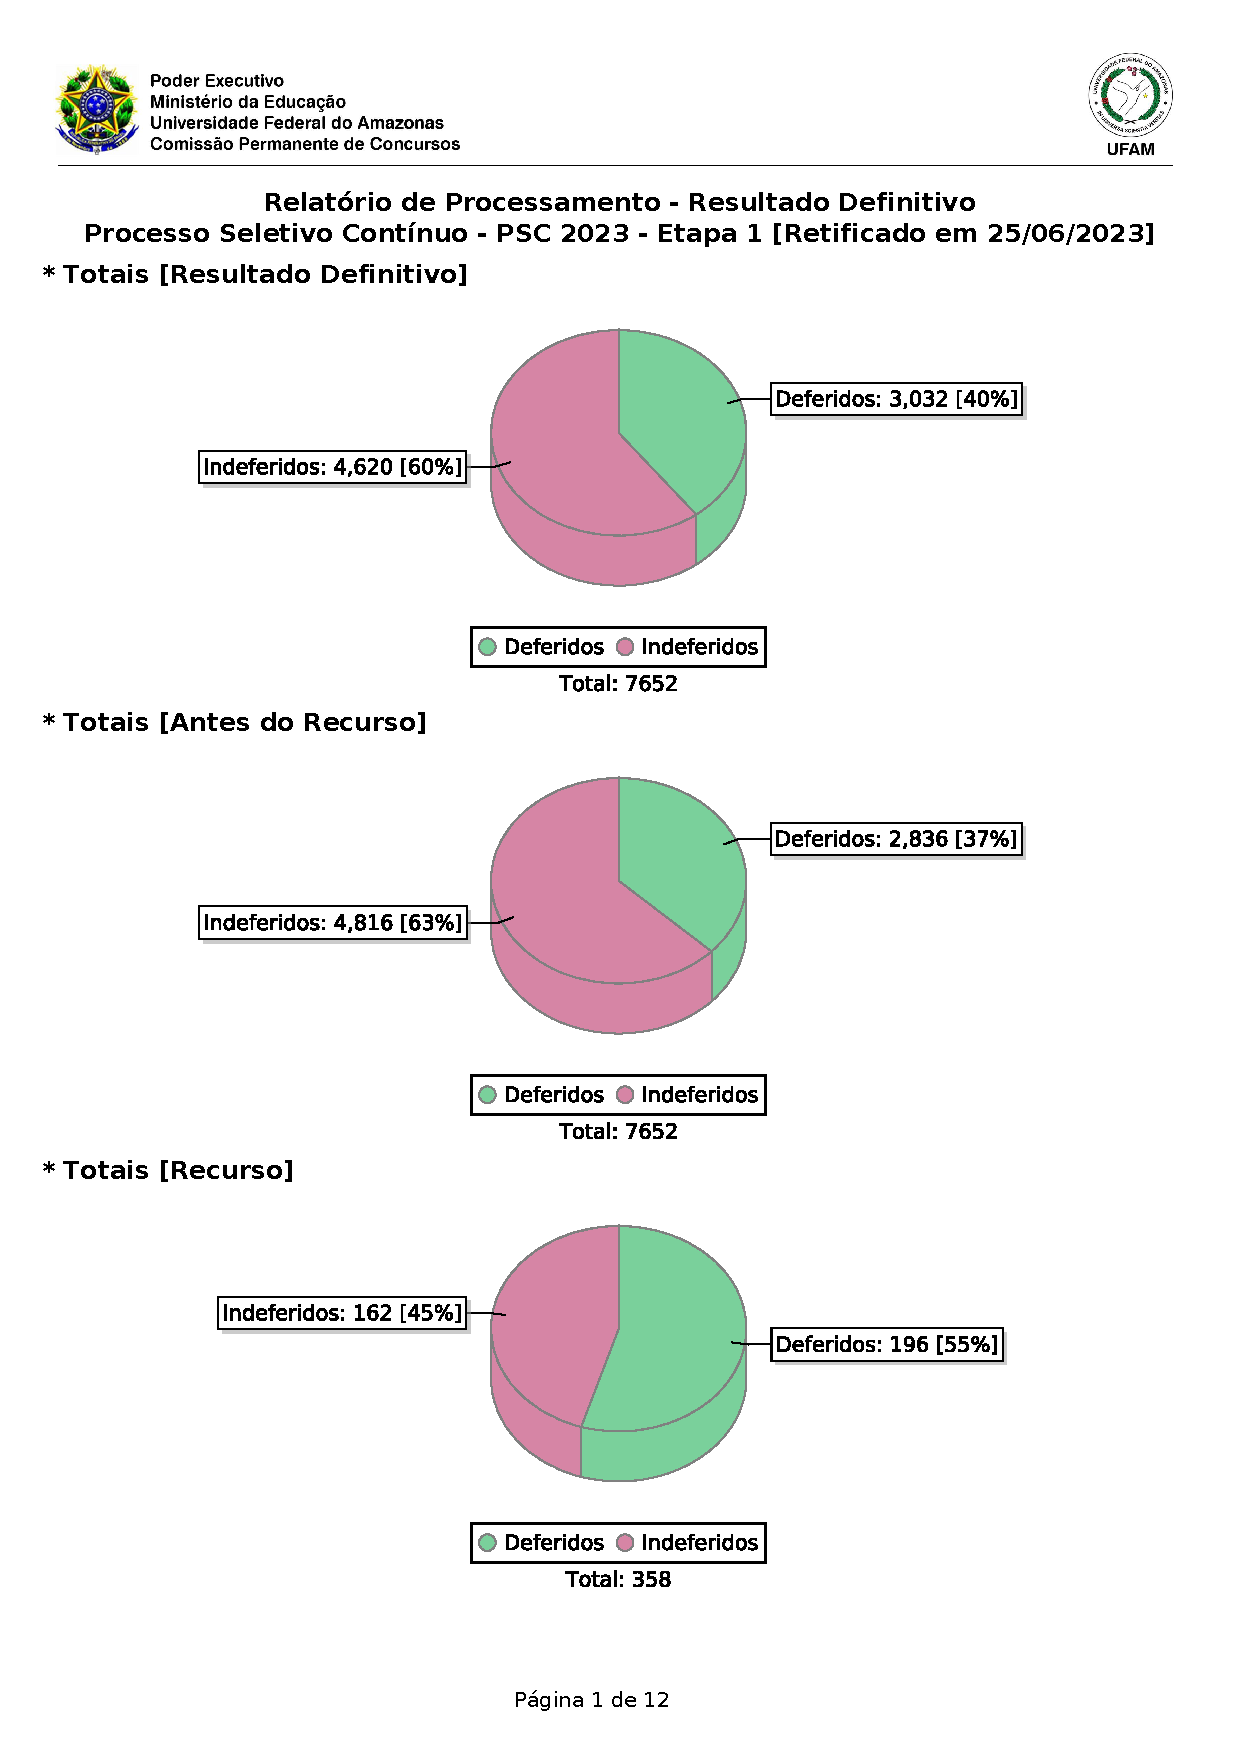
\includepdf[pages=-,pagecommand={},width=175 mm]{anexos/psc2023-e12-relatorio-processamento}
		
	\end{anexosenv}

\end{document}